\chapter{Design Dettagliato}

In questo capitolo andremo piu' a basso livello elencando le tecnologie che saranno utilizzate e
definiremo meglio la struttura del db, interazioni e degli algoritmi di cifratura.

\section{Tecnologie utilizzate}

\subsection{Linguaggio}
Ho deciso di fare tutto in Python per diversi motivi:
\begin{itemize}
    \item Gestione automatica dei BigInt, questo mi permette di gestire facilmente le cifrature
    asimmetriche.
    \item Facile creazione e modifica di database.
    \item Facile utilizzo di TCP socket.
    \item Conoscenza pregressa.
\end{itemize}
Sicuramente questa scelta ha molti contro che avrei valutato se fosse un progetto di lavoro o che
comunque dovesse diventare di dominio e utilizzo pubblico. In particolare ovviamente il punto
dolente e' la lentezza di esecuzione.

Nonostante Python abbia una fantastica libreria (Pycryptodome) ho deciso di non utilizzarla ma di
implementare a mano tutti gli algoritmi. Questo e' il motivo principale che mi ha portato a
preferire algoritmi meno sicuri ma piu' semplici da implementare.

\section{Cifratura}

Nello scambio di chiavi con il server sara' utilizzata una cifratura ibrida che unisce Diffie Hellman e
RSA. Ho scelto di fare in questo modo perche' non volevo che il sistema fosse vulnerabile al MITM
attack. Infatti se usassi solo diffie hellman potrei avere problemi se un attaccante si immettesse
nella comunicazione. Invece utilizzando anche RSA per firmare i messaggi evito questo problema e
inoltre garantisco forward secrecy in caso la chiave RSA fosse compromessa. Una
volta scambiate le chiavi private la cifratura avverra' tramite DES che pur non essendo sicuro e'
piu' semplice da implementare visto che ho deciso di non usare librerie crittografiche.

\subsection{Dettaglio}

\subsubsection{RSA}

\begin{figure}[H]
    \centering{}
    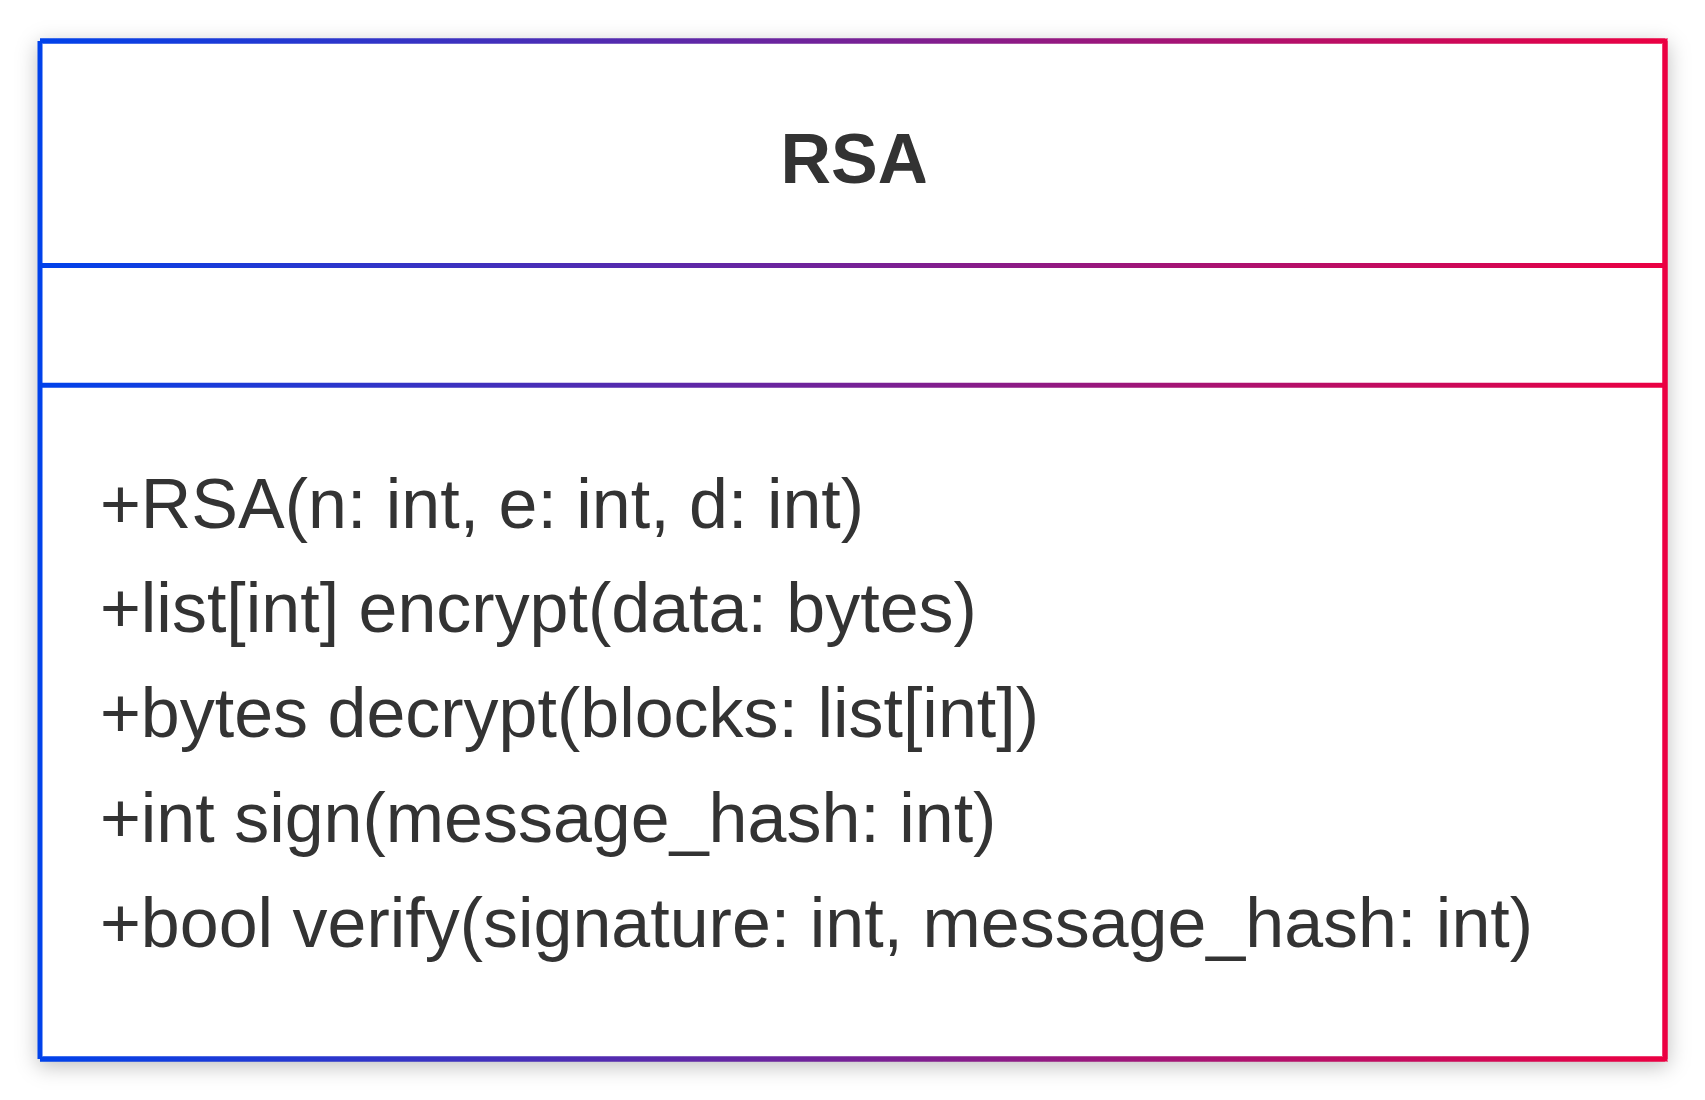
\includegraphics[width=.8\textwidth]{img/class/RSA.png}
    \caption{Diagramma della classe RSA.}
    \label{class:RSA}
\end{figure}

Come si vede in \ref{class:RSA}, la classe RSA e' molto semplice e contiene le funzioni che ci
serviranno, quindi cifratura, decifratura, firma e verifica della firma.
Per RSA verranno utilizzate chiavi a 2048 bit. La chiave del server e' nota a priori ai client per
evitare l'utilizzo di certificati.

\subsubsection{Diffie Hellman}

\begin{figure}[H]
    \centering{}
    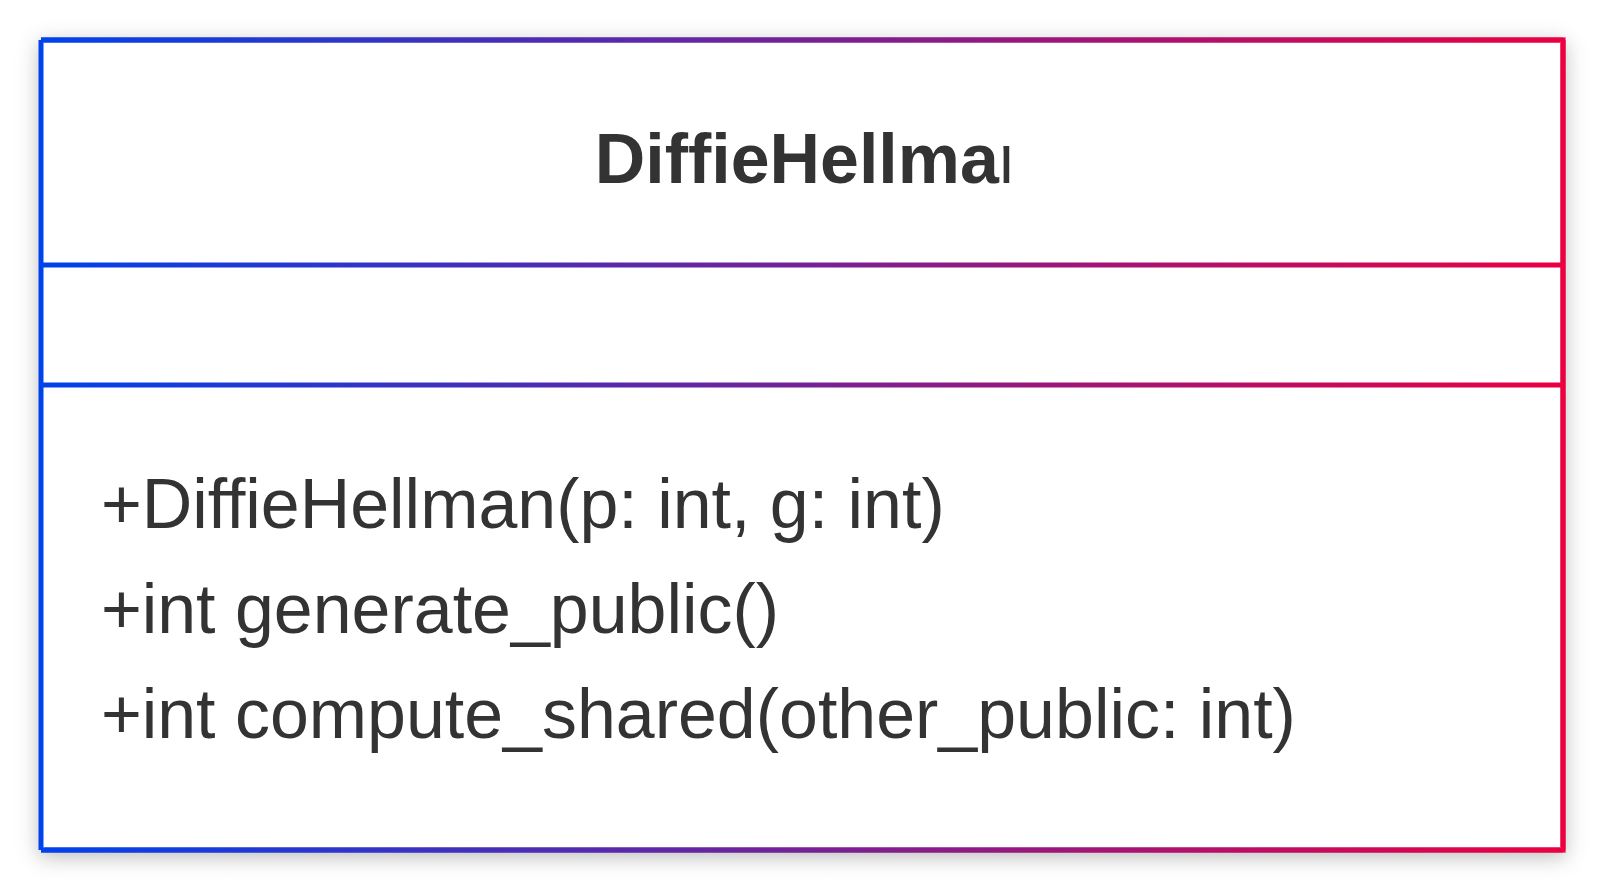
\includegraphics[width=.8\textwidth]{img/class/DH.png}
    \caption{Diagramma della classe Diffie Hellman.}
    \label{class:DH}
\end{figure}

Anche in questo caso la classe e' molto semplice e contiene le funzioni per generare la chiave
pubblica e ottenere la chiave condivisa.
Per Diffie Hellman verranno utilizzate chiavi a 2048 bit. I valori di g e p sono fissati per ogni
scambio.

\subsubsection{Generazione numeri primi}
I numeri primi saranno generati sfruttando il teorema di Fermat visto a lezione, quindi prendendo un
numero casuale e testandone la primalita' in modo probabilistico. A lezione abbiamo visto che con un
numero di 100 cifre la probabilita' di sbagliare e' minuscola e le chiavi a 2048 bit hanno circa 600
cifre quindi siamo abbastanza tranquilli. Non usero' il test di primalita' probabilistico esteso
perche' non lo trovo necessario in questo caso avendo numeri molto grandi.
Per la generazione di numeri random grandi usero' getrandbits della libreria
\href{https://docs.python.org/3/library/secrets.html}{secrets} che usa un algoritmo
sicuro crittograficamente.

\subsubsection{DES}

\begin{figure}[H]
    \centering{}
    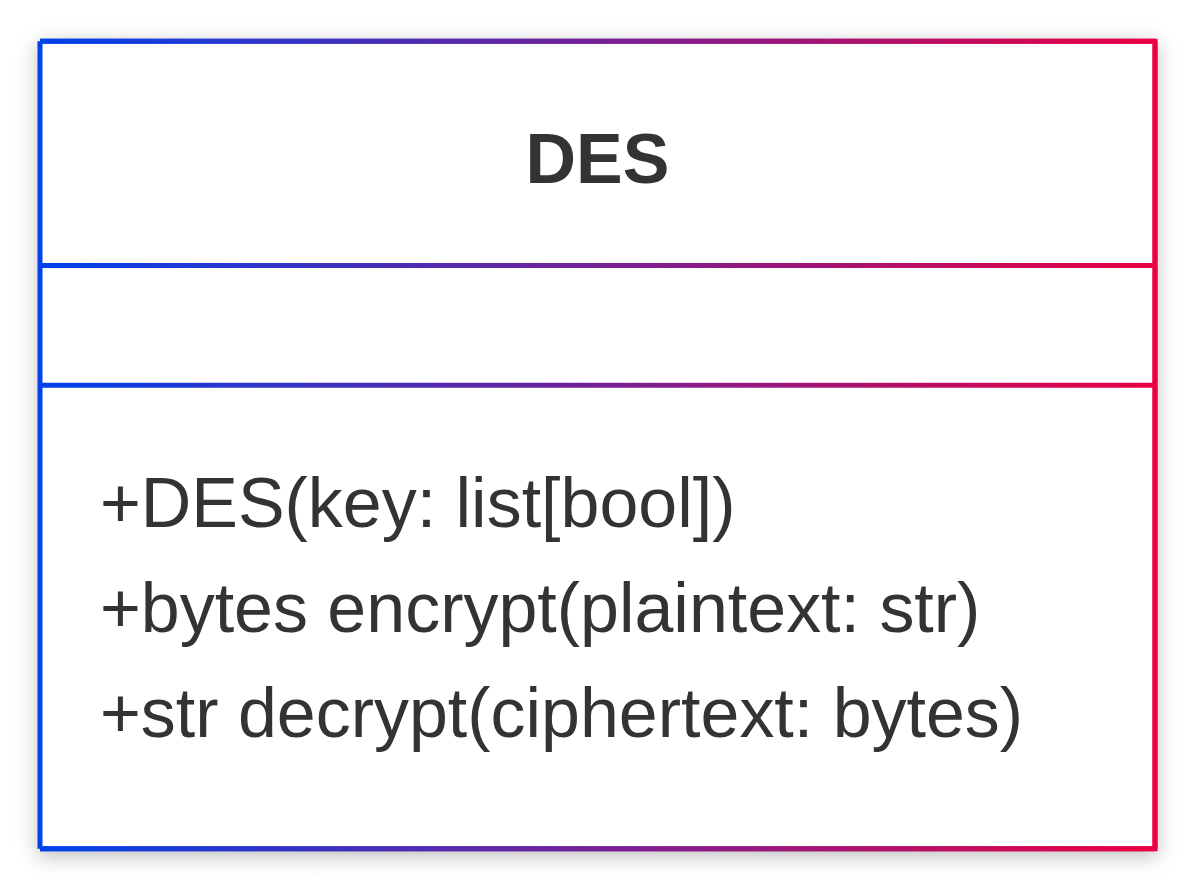
\includegraphics[width=.8\textwidth]{img/class/DES.png}
    \caption{Diagramma della classe DES.}
    \label{class:DH}
\end{figure}

La classe DES permette, data la chiave, di cifrare e decifrare i messaggi. Per l'implementazione mi
sono basato sulle indicazioni date \href{https://en.wikipedia.org/wiki/Data_Encryption_Standard}{qui}
e le tabelle sono state prese \href{https://en.wikipedia.org/wiki/DES_supplementary_material}{qui}.

\section{Interazioni}
Per la comunicazione usero' il protocollo TCP con la libreria
\href{https://docs.python.org/3/library/socket.html}{socket} in quanto voglio avere la garanzia
dell'arrivo corretto dei messaggi.

\subsection{Tipologia di messaggi}

\begin{figure}[H]
    \centering{}
    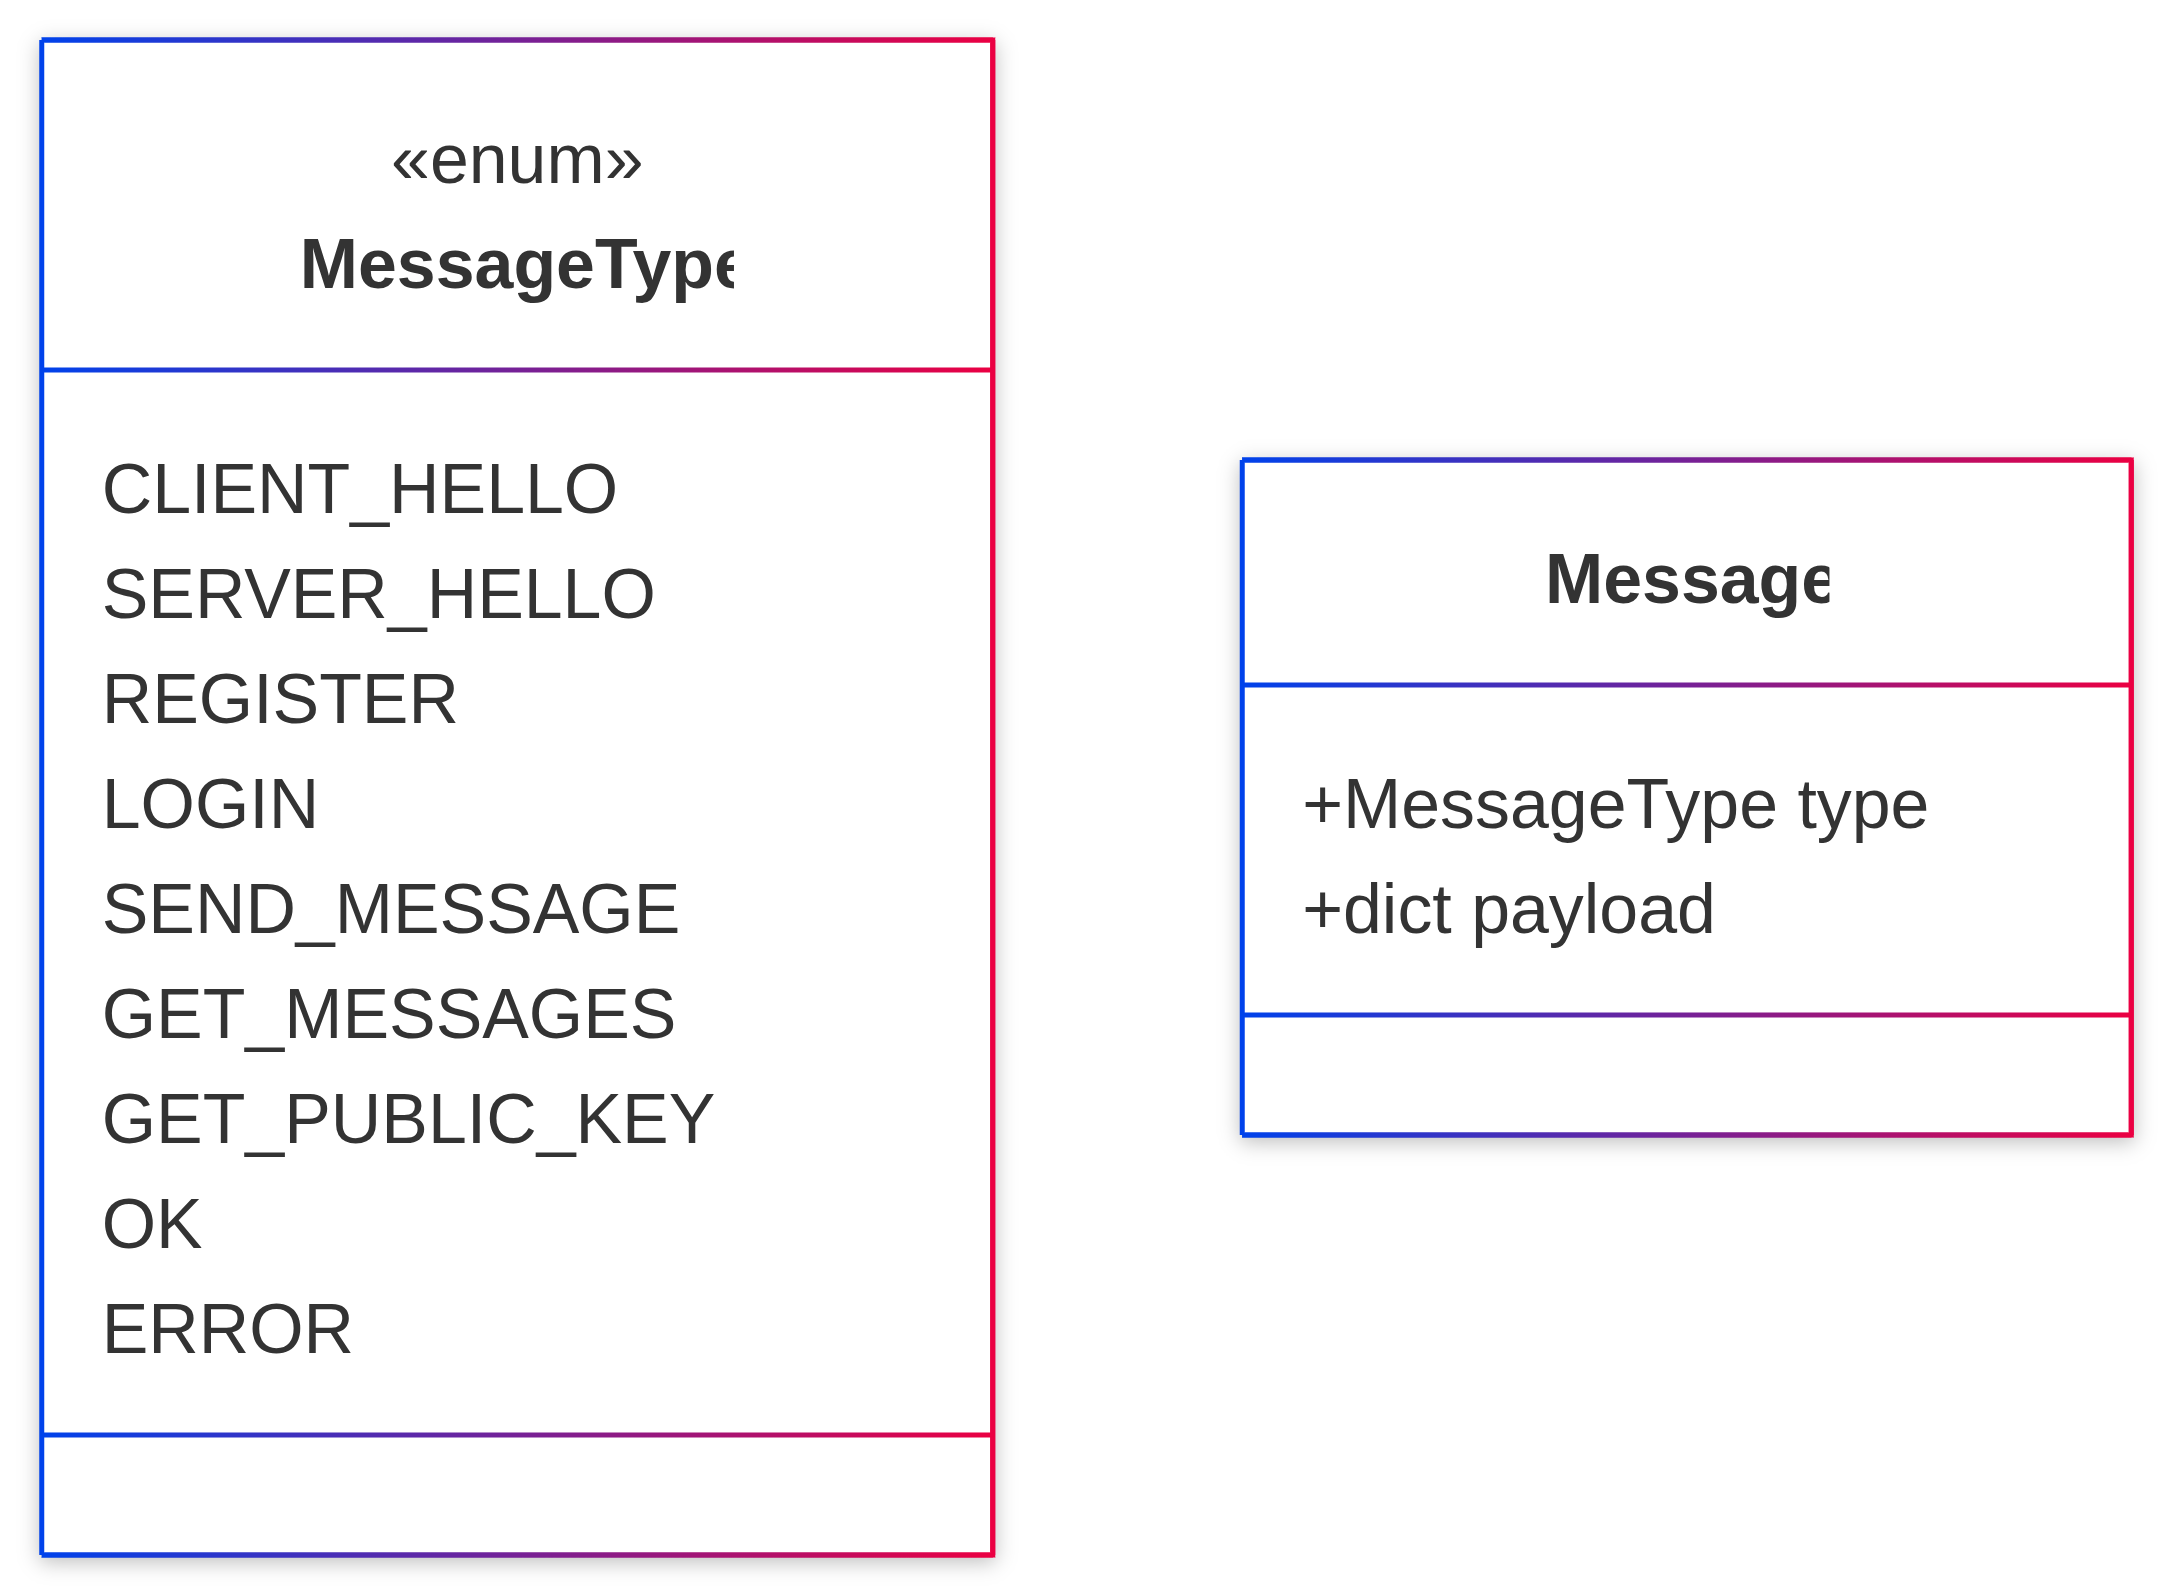
\includegraphics[width=.8\textwidth]{img/class/Messages.png}
    \caption{Diagramma della classe Message e MessageType.}
    \label{class:Messages}
\end{figure}

Come si vede in \ref{class:Messages} ci sono diversi tipi di messaggi:
\begin{itemize}
    \item CLIENT\_HELLO: il primo messaggio che il client manda al server per iniziare l'handshake.
    \item SERVER\_HELLO: la risposta del server che conclude lo scambio di chiavi.
    \item REGISTER: inviato dal client per registrare un nuovo utente fornendo username e password.
    \item LOGIN: inviato dal client per eseguire il login fornendo username e password.
    \item SEND\_MESSAGE: usato per l'invio di un messaggio client-client.
    \item GET\_MESSAGES: usato per ottenere dal server tutti i messaggi non ancora ricevuti.
    \item GET\_PUBLIC\_KEY: usato dal client per ottenere la public key di qualcun altro dato l'username.
    \item OK: usato come risposta del server per confermare la corretta esecuzione di un'azione.
    \item ERROR: usato come risposta del server per segnalare un errore durante l'esecuzione di un'azione.
\end{itemize}

In \ref{class:Messages} si vede anche la semplice struttura del messaggio che conterra' il tipo e il
contenuto come dizionario.

\subsection{Protocollo scambio di chiavi}
In questa sezione vedremo la tipologia messaggi scambiati per le comunicazioni.

\subsubsection{Scambio tra client e server}

\begin{figure}[H]
    \centering{}
    \includegraphics[width=\textwidth]{img/sequenza/client\_server\_hello.png}
    \caption{Diagramma di sequenza messaggi HELLO.}
    \label{seq:hello}
\end{figure}

Come si vede in \ref{seq:hello}:
\begin{itemize}
    \item Il client invia un messaggio CLIENT\_HELLO con la chiave pubblica A per DH, la chiave
    pubblica RSA e la firma di tutto il payload.
    \item Il server risponde con SERVER\_HELLO con l'altra parte di chiave B per DH e la firma. La
    firma ovviamente contiene anche A perche' il client deve essere sicuro della corretta ricezione
    da parte del server.
    \item Il client verifica la firma ed entrambi calcolano la chiave condivisa e puo' iniziare la
    comunicazione cifrata con DES.
\end{itemize}

\begin{figure}[H]
    \centering{}
    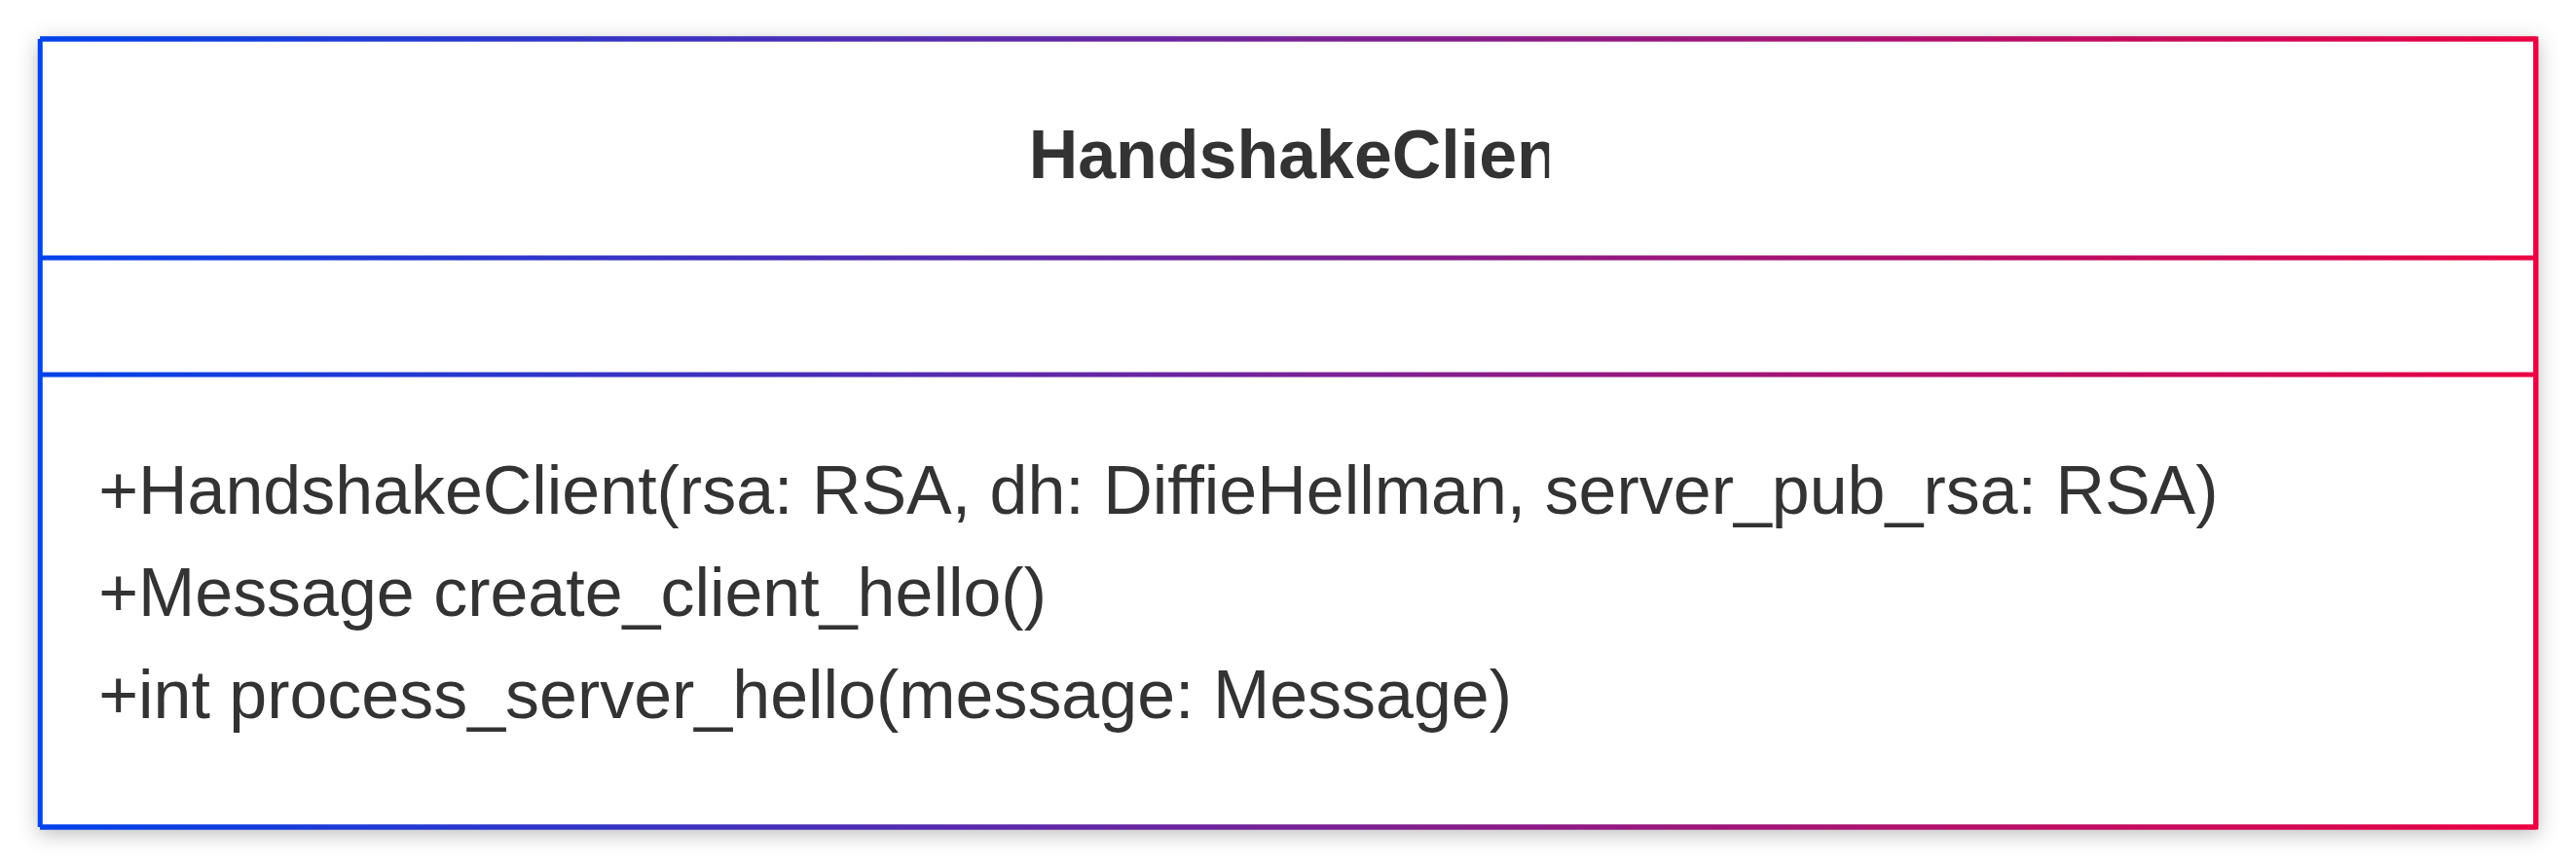
\includegraphics[width=.8\textwidth]{img/class/HandshakeClient.png}
    \caption{Diagramma della classe HandshakeClient.}
    \label{class:HandshakeClient}
\end{figure}

\begin{figure}[H]
    \centering{}
    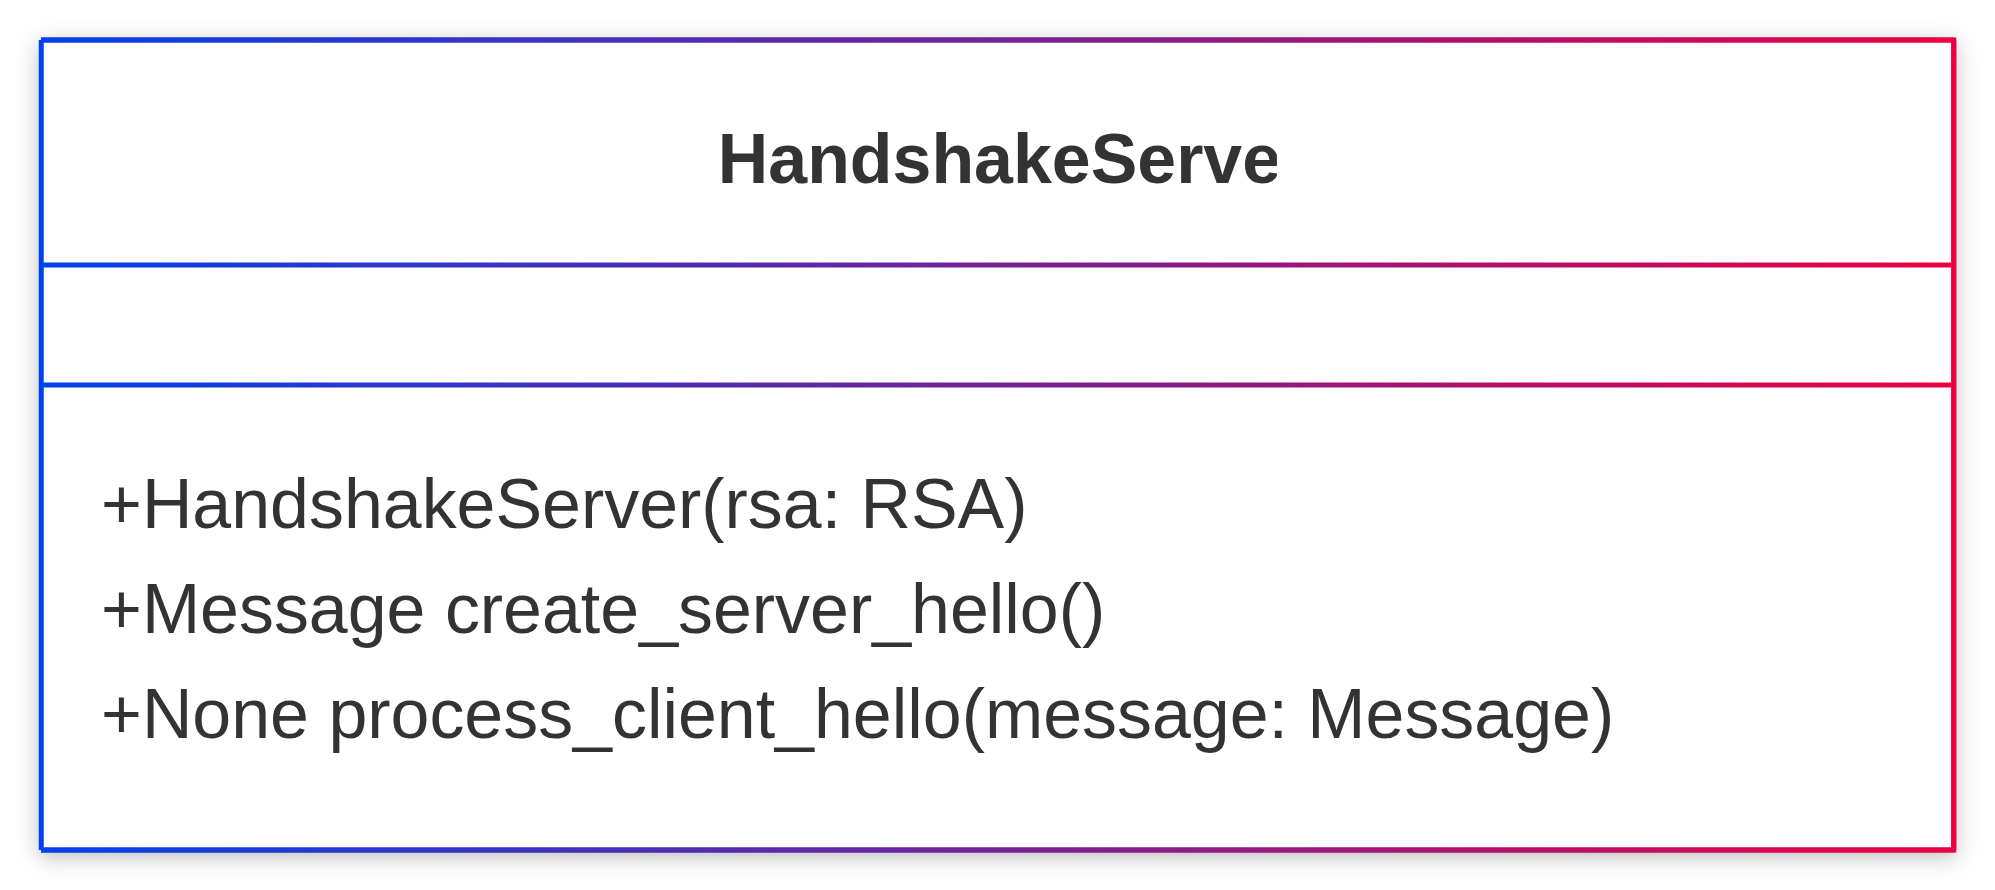
\includegraphics[width=.8\textwidth]{img/class/HandshakeServer.png}
    \caption{Diagramma della classe HandshakeServer.}
    \label{class:HandshakeServer}
\end{figure}

Le classi \ref{class:HandshakeClient} e \ref{class:HandshakeServer} servono proprio per gestire lo
scambio di chiavi usando DiffieHellman e verificando le firme.

\subsubsection{Registrazione}

\begin{figure}[H]
    \centering{}
    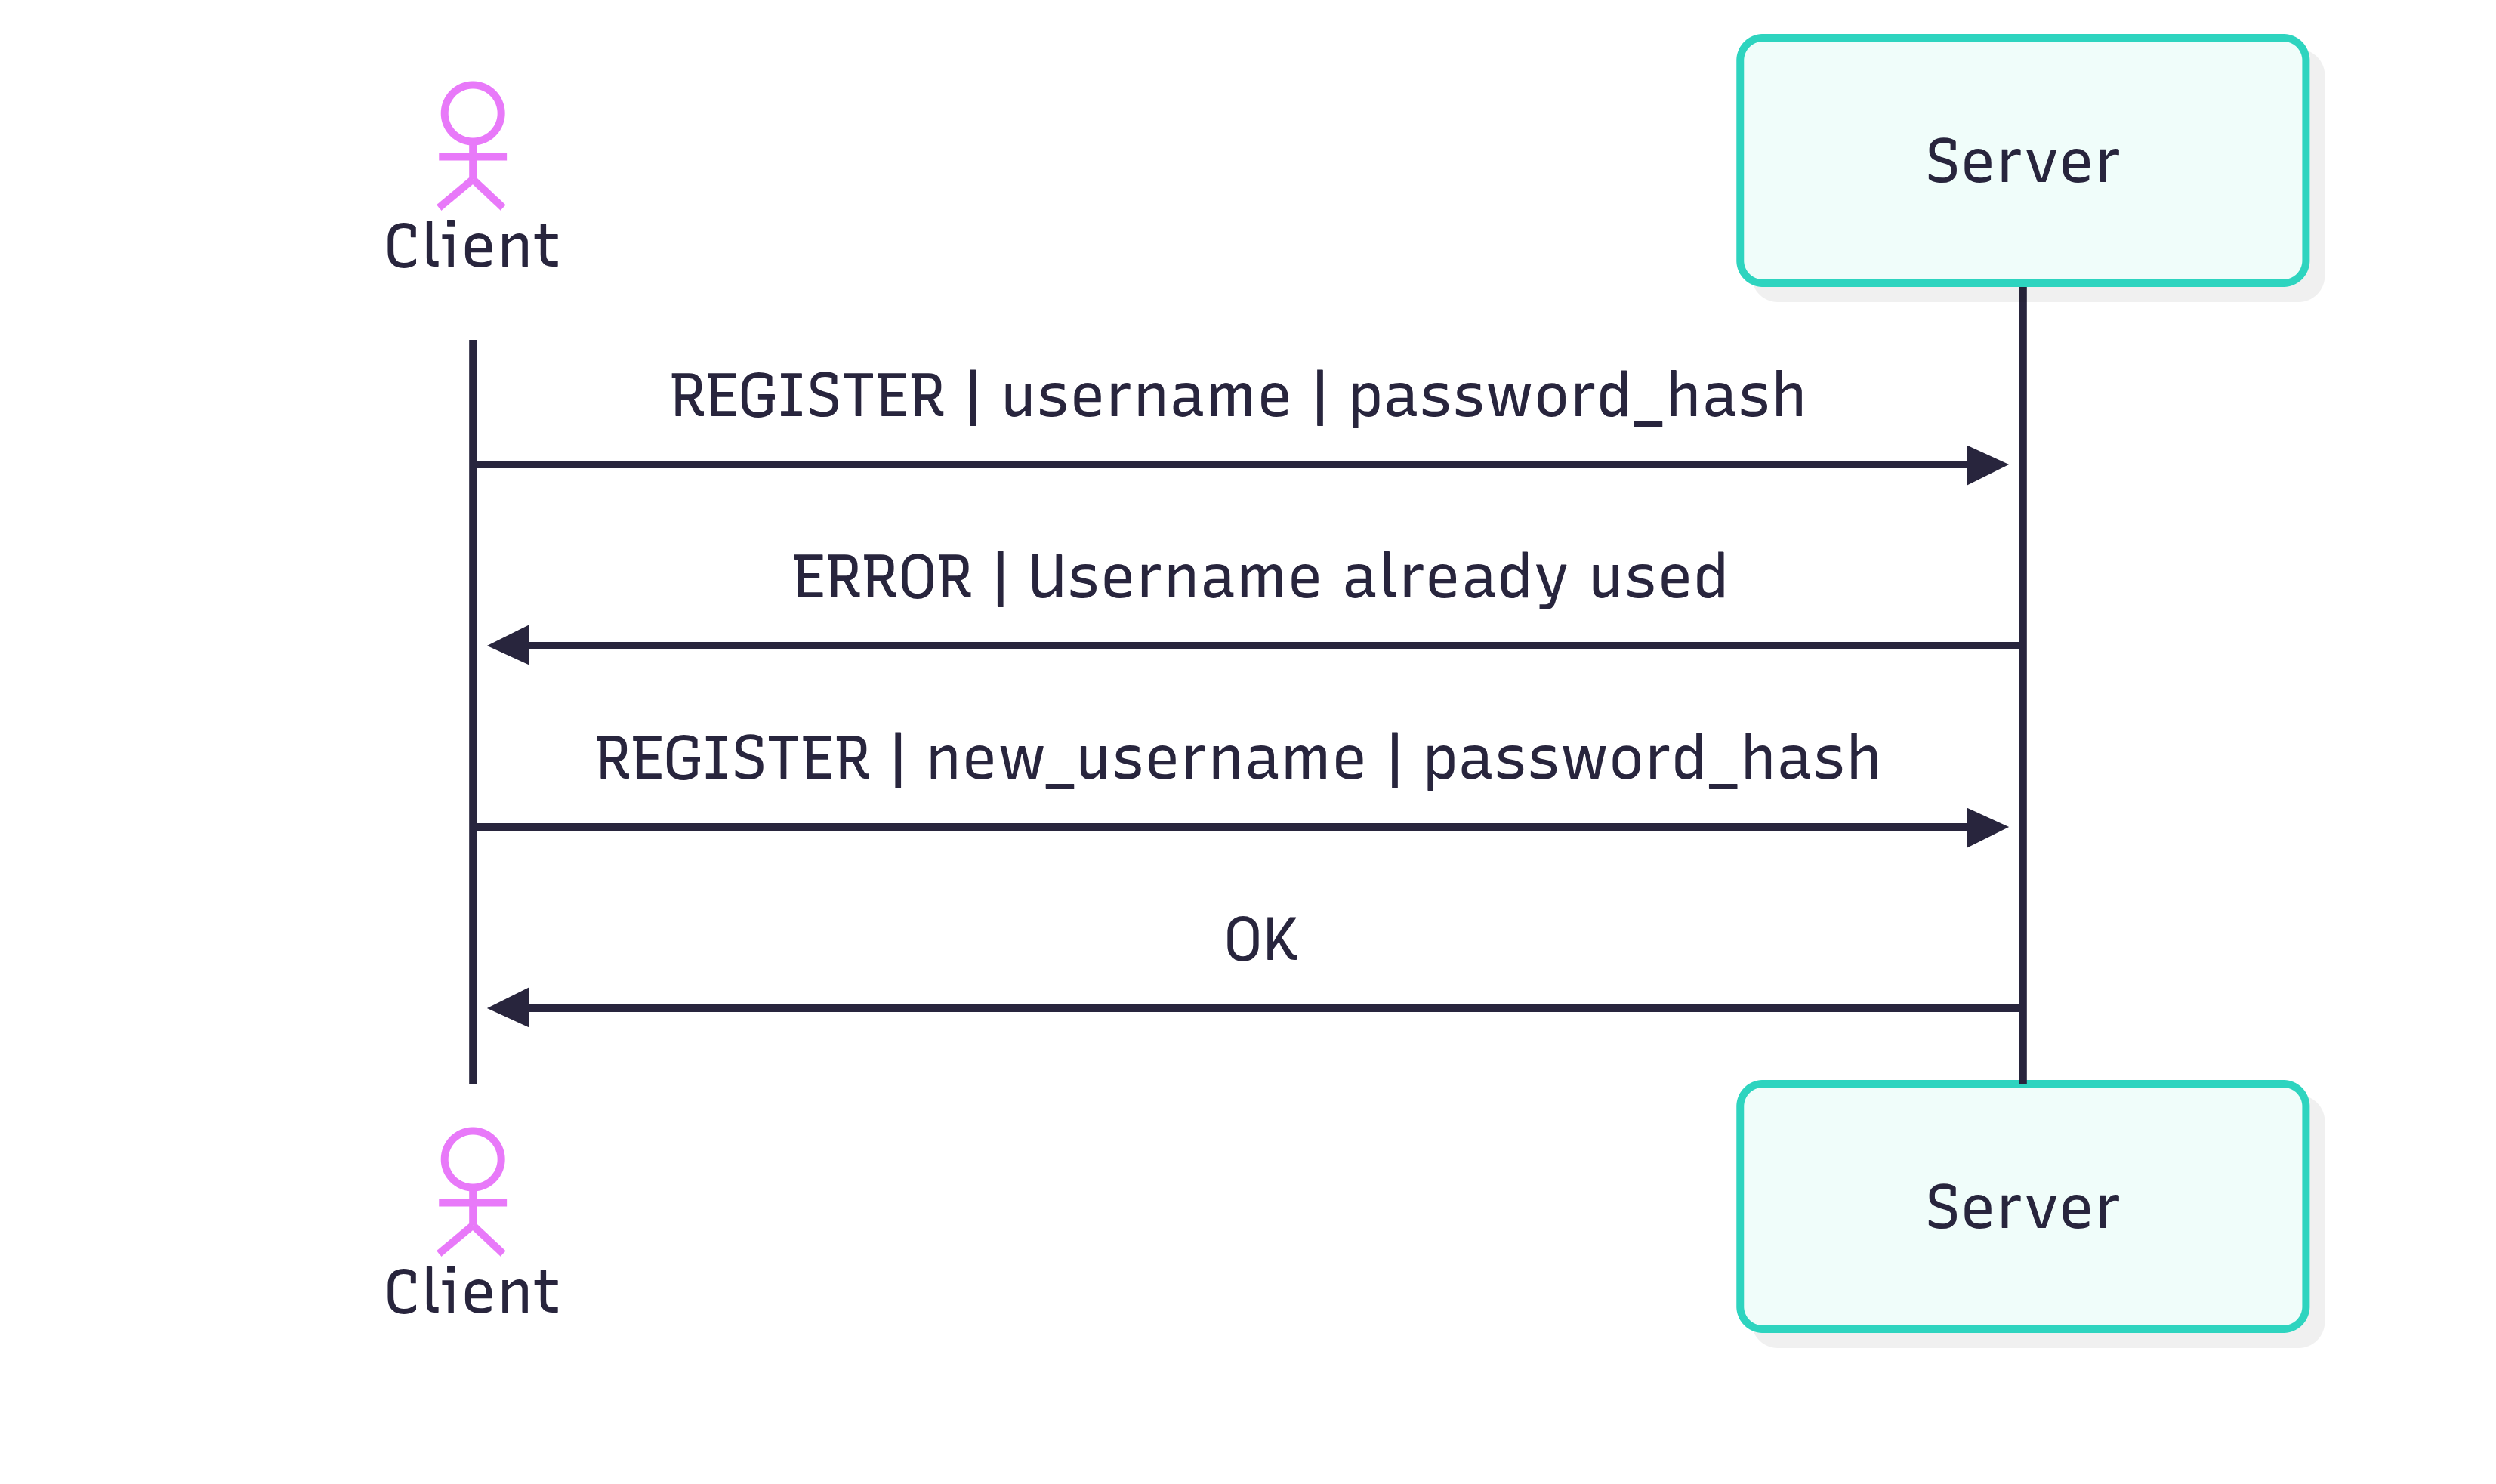
\includegraphics[width=\textwidth]{img/sequenza/register.png}
    \caption{Diagramma di sequenza REGISTER.}
    \label{seq:register}
\end{figure}

Come si vede in \ref{seq:register}, una volta scambiate le chiavi il client invia il messaggio
REGISTER con username e password\_hash. Il server salvera' tutti i dati dopo aver controllato che l'username sia
univoco e poi rispondera' con OK oppure con ERROR con l'errore riscontrato.

\subsubsection{Login}

\begin{figure}[H]
    \centering{}
    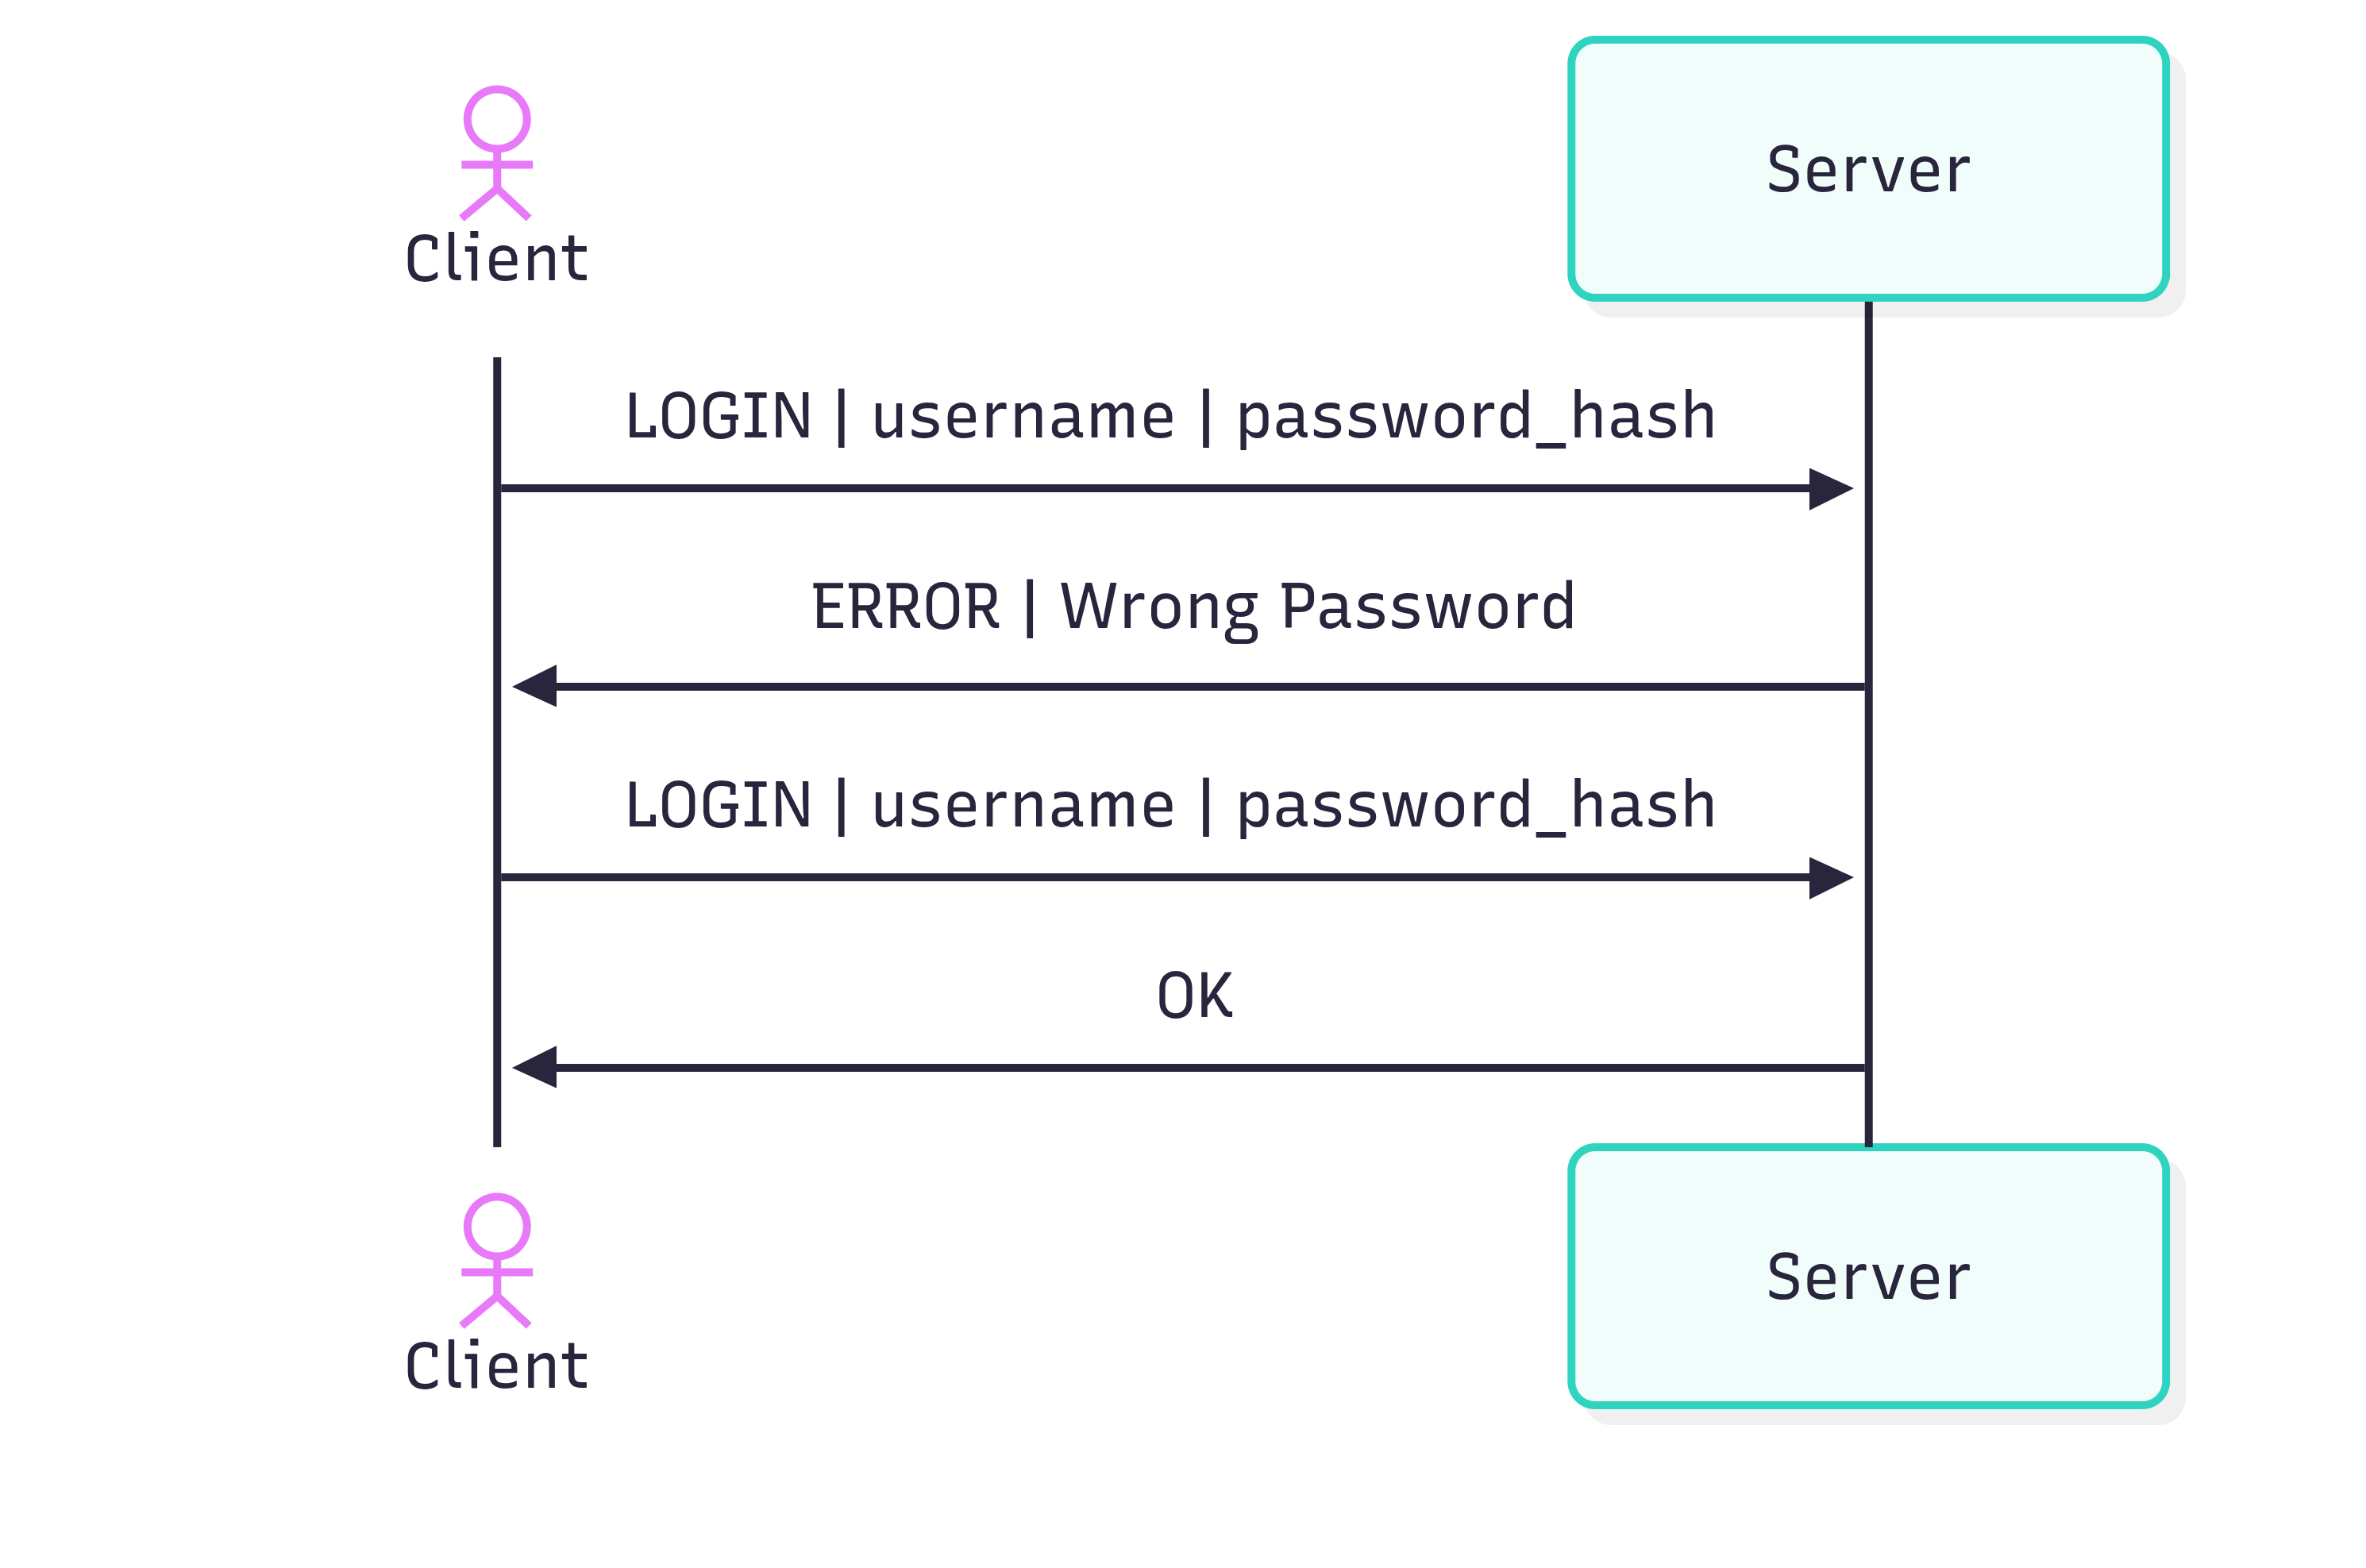
\includegraphics[width=\textwidth]{img/sequenza/login.png}
    \caption{Diagramma di sequenza LOGIN.}
    \label{seq:login}
\end{figure}

Come si vede in \ref{seq:login}, per il login il client inviera' un messaggio LOGIN con username e password\_hash e il server
rispondera' con OK oppure con ERROR con l'errore riscontrato.

\subsubsection{Comunicazione tra client}

\begin{figure}[H]
    \centering{}
    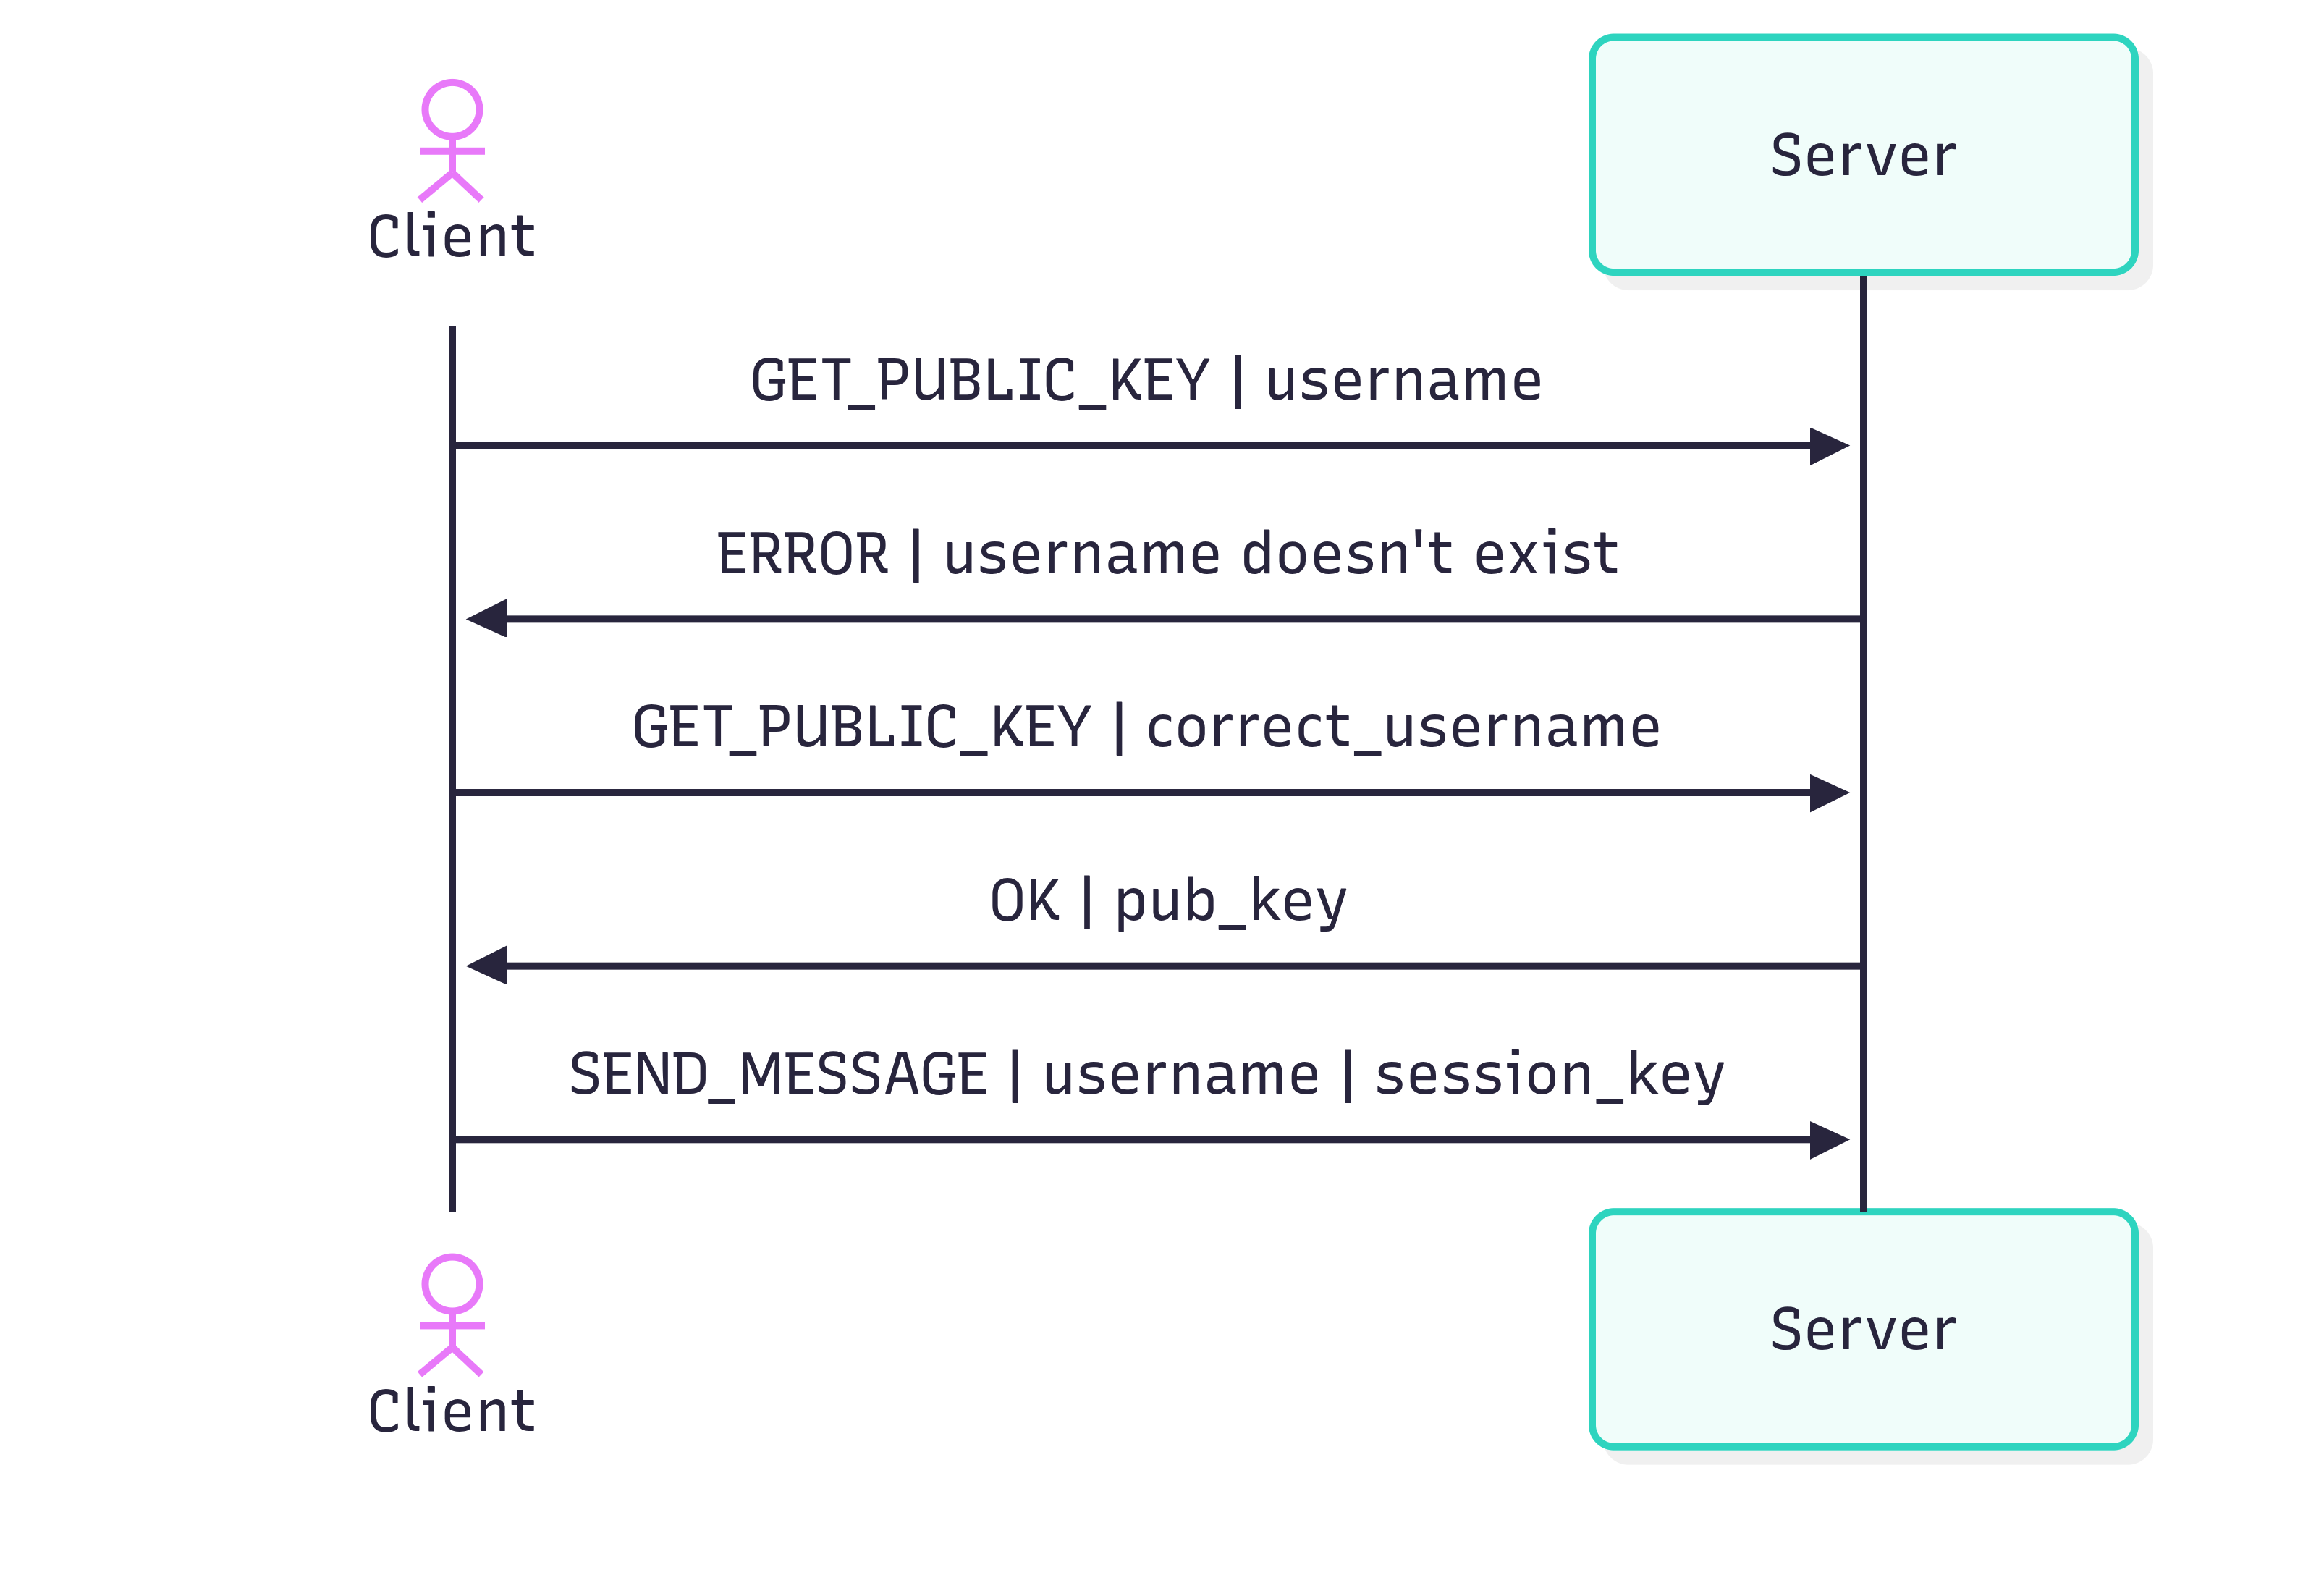
\includegraphics[width=\textwidth]{img/sequenza/get_public_key.png}
    \caption{Diagramma di sequenza GET\_PUBLIC\_KEY.}
    \label{seq:get_public_key}
\end{figure}

Come si vede in \ref{seq:get_public_key}, per la comunicazione tra client il server agisce solo come tramite dei messaggi. Il client inviera'
un messaggio GET\_PUBLIC\_KEY con l'username dell'utente interessato e il server rispondera' con un
messaggio OK e la chiave pubblica dell'utente oppure con ERROR se c'e' stato
qualche errore. Successivamente il client genera una chiave simmetrica e la invia cifrata con la
chiave pubblica del destinatario nel messaggio SEND\_MESSAGE che contiene il destinatario e la
chiave simmetrica cifrata.

\subsubsection{Invio e richiesta messaggi}

\begin{figure}[H]
    \centering{}
    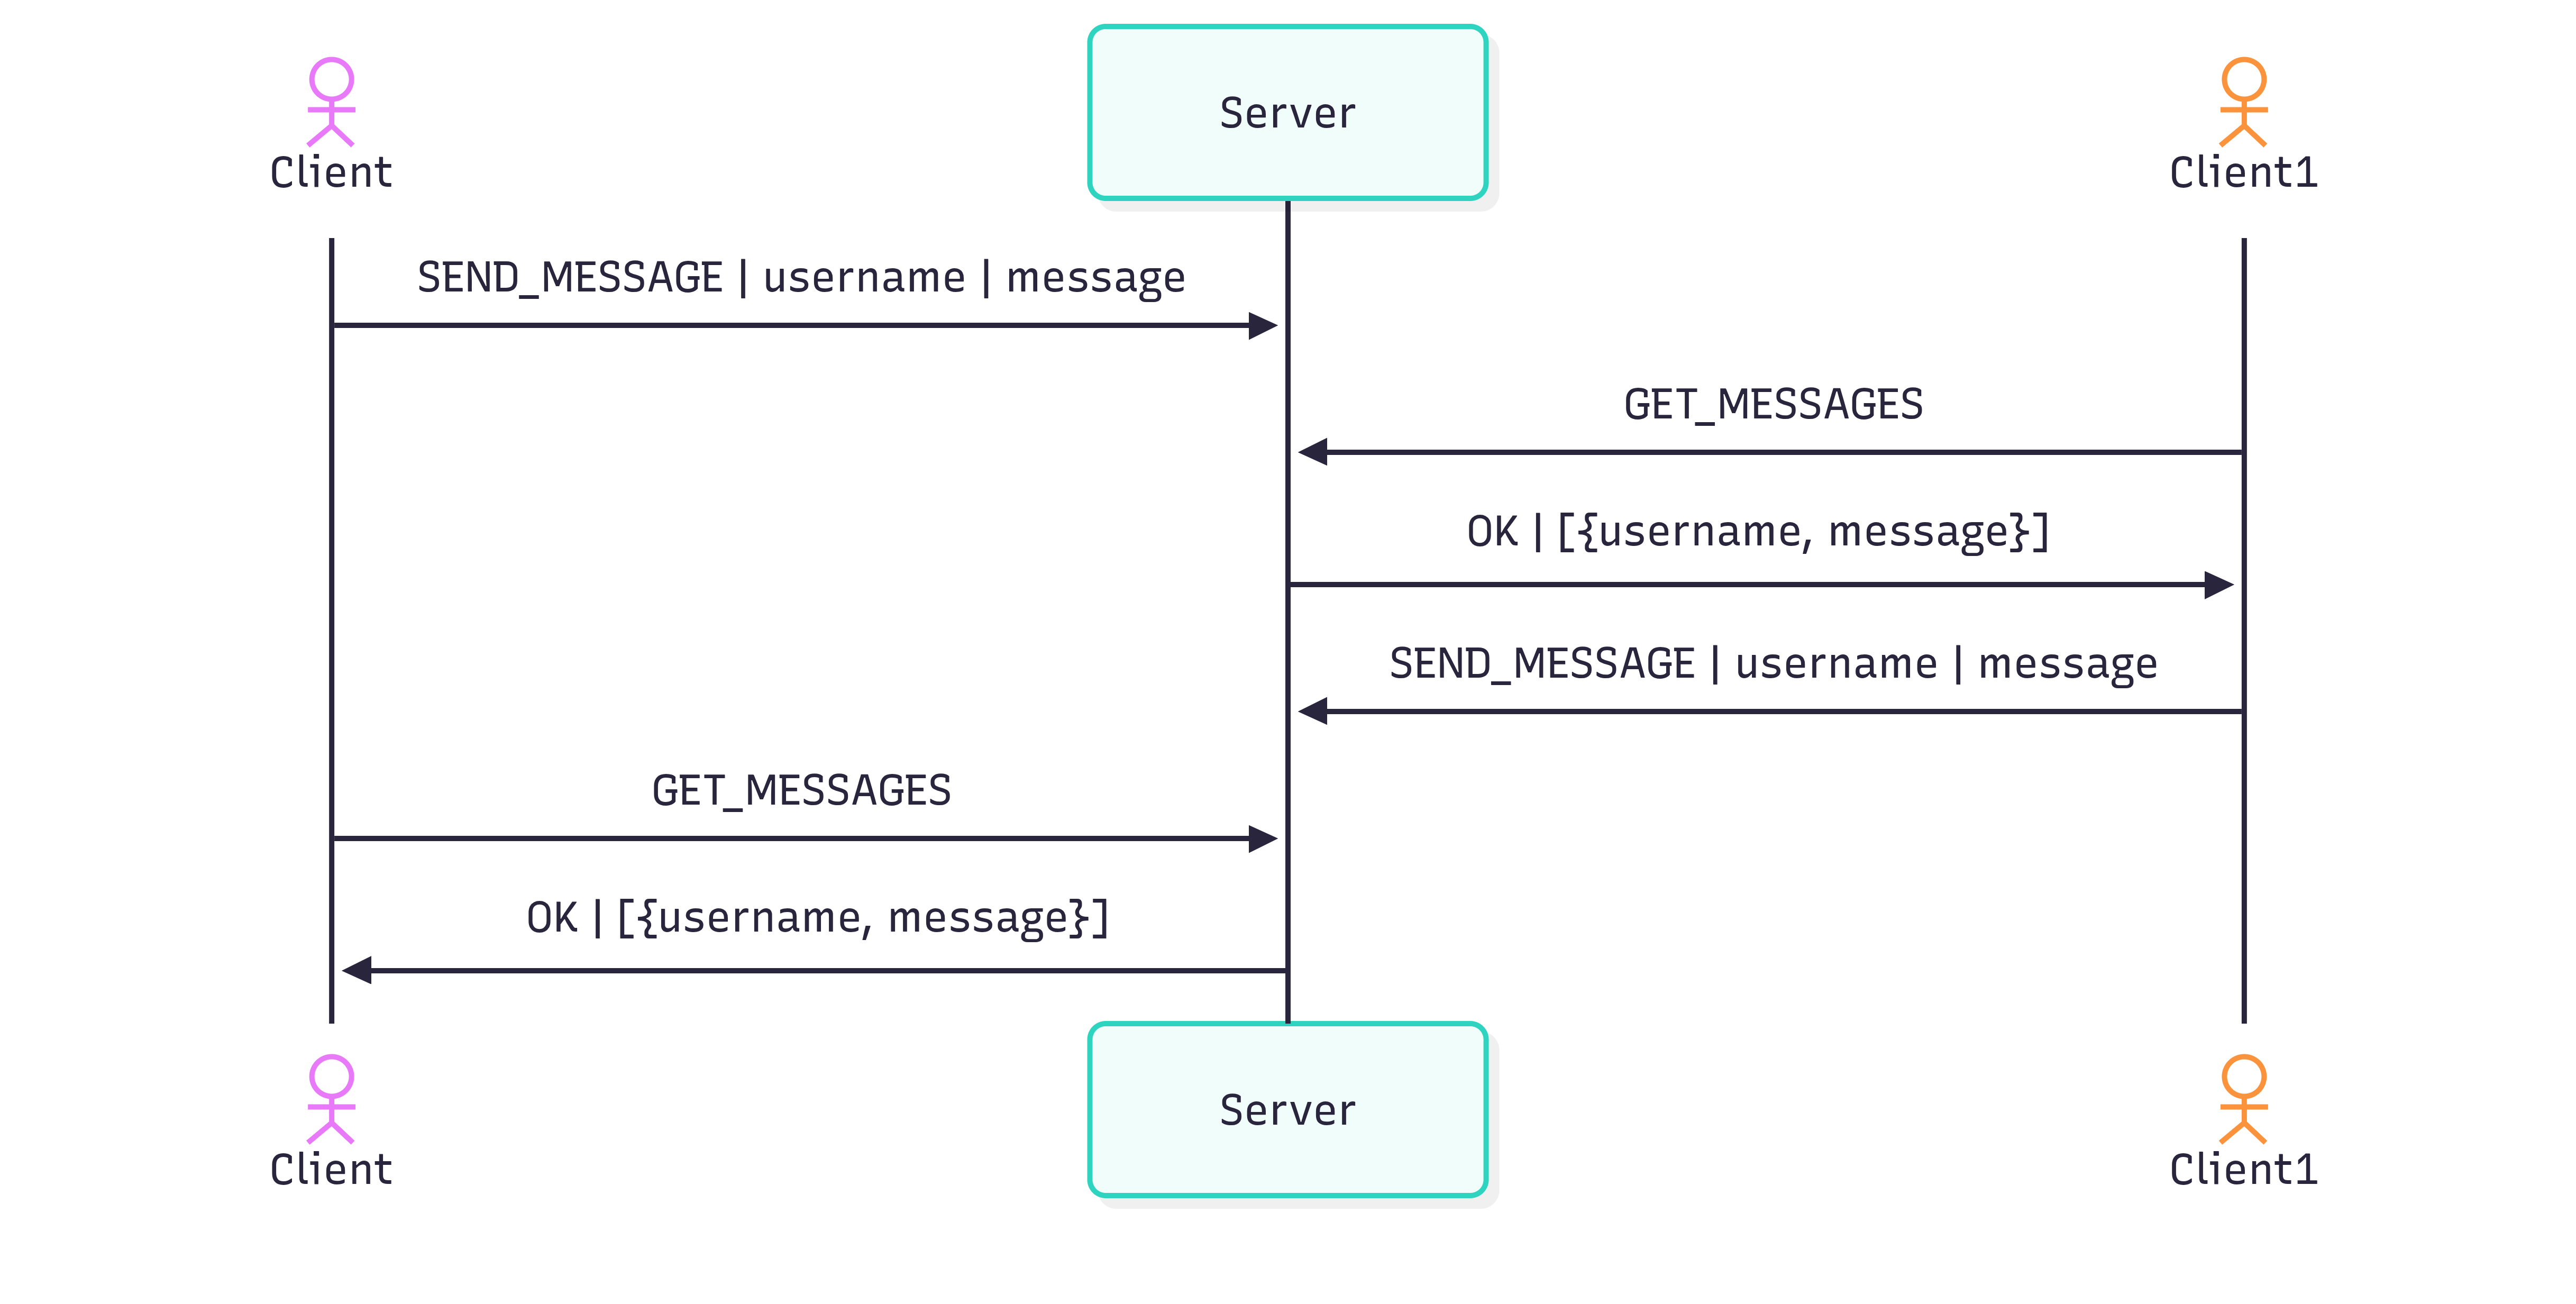
\includegraphics[width=\textwidth]{img/sequenza/send_get_messages.png}
    \caption{Diagramma di sequenza invio e richiesta messaggi.}
    \label{seq:send_get_message}
\end{figure}

Come si vede in \ref{seq:send_get_message}, una volta eseguito il tutto i messaggi saranno della
forma SEND\_MESSAGE con destinatario e messaggio cifrato tramite DES. I client periodicamente inviano
un messaggio GET\_MESSAGES al server che rispondera' con un messaggio OK contentente tutti i
messaggi nuovi.

\section{Database}

\subsection{Tecnologie}
Per i database ho deciso di utilizzare semplici file .db con la libreria sqlite3, in questo modo ho
tutto integrato in Python ed e' piu' semplice l'implementazione.

\subsection{Server}

\begin{figure}[H]
    \centering{}
    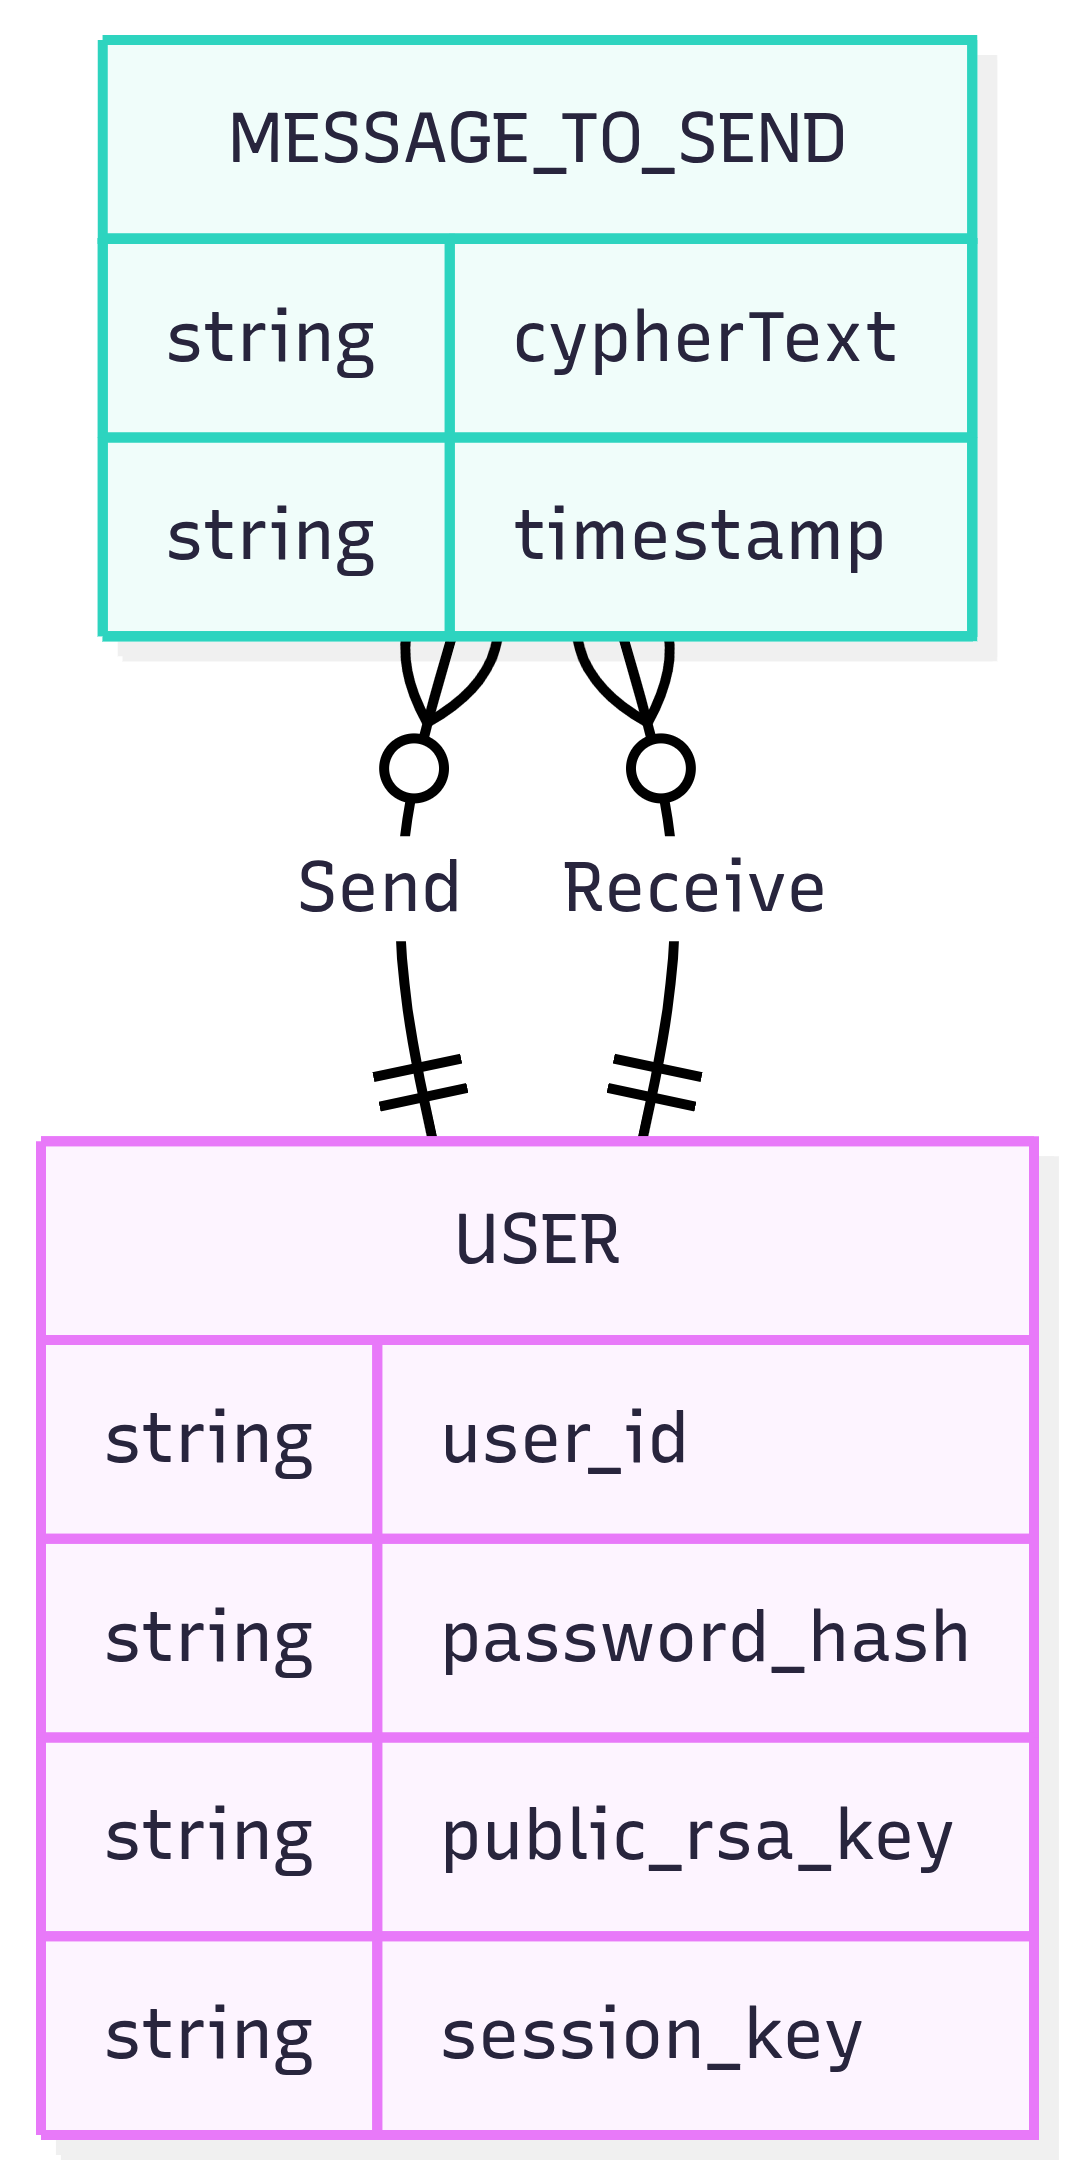
\includegraphics[width=.4\textwidth]{img/er/server_users_messages.png}
    \caption{Diagramma er database del server.}
    \label{er:server_db}
\end{figure}

Come si vede in \ref{er:server_db} abbiamo 2 entita', una per gli utenti che sono identificati
dall'id e contengono l'hash della password e le eventuali chiavi di sessione oppure pubbliche RSA.
Ovviamente teniamo l'hash e non la password in chiaro perche' non vogliamo che il server conosca la
password degli utenti.
Il server manterra' anche i messaggi che non sono stati ancora ricevuti dai client e di questi ci
interessa mittente, destinatario e ovviamente il messaggio cifrato con la chiave privata scambiata
dagli utenti in modo che il server non possa leggere i messaggi ma faccia solo da tramite. Una volta
ricevuto il comando GET\_MESSAGES il server eliminera' dal database i messaggi.

\subsubsection{Password Hashing}
Ogni password subira' 2 hashing. Uno lato client per fare in modo che nella comunicazione non passi
la password in chiaro. Per fare questo utilizzo sha256 con un salt che e' fisso ed e' l'username.
In questo modo vengono nascoste le password identiche ad eventuali attaccanti e inoltre ogni
attaccante dovrebbe creare tabelle diverse per ogni utente se volesse cercare di ottenere le
password.

Lato server viene eseguito un ulteriore hashing utilizzando PBKDF2-HMAC-SHA256 con salt casuale e
100 000 iterazioni. In questo modo risulta molto difficile, anche avendo il db, trovare le password
velocemente perche' la computazione dell'hash non puo' essere fatta in modo rapido come un banale
sha256. Ho deciso di non utilizzare Argon2 pur essendo piu' moderno perche' avrei docuto installare
la libreria apposita, invece PBKDF2 e' gia' presente nella libreria
\href{https://docs.python.org/3/library/hashlib.html}{hashlib}.

\subsection{Client}

\begin{figure}[H]
    \centering{}
    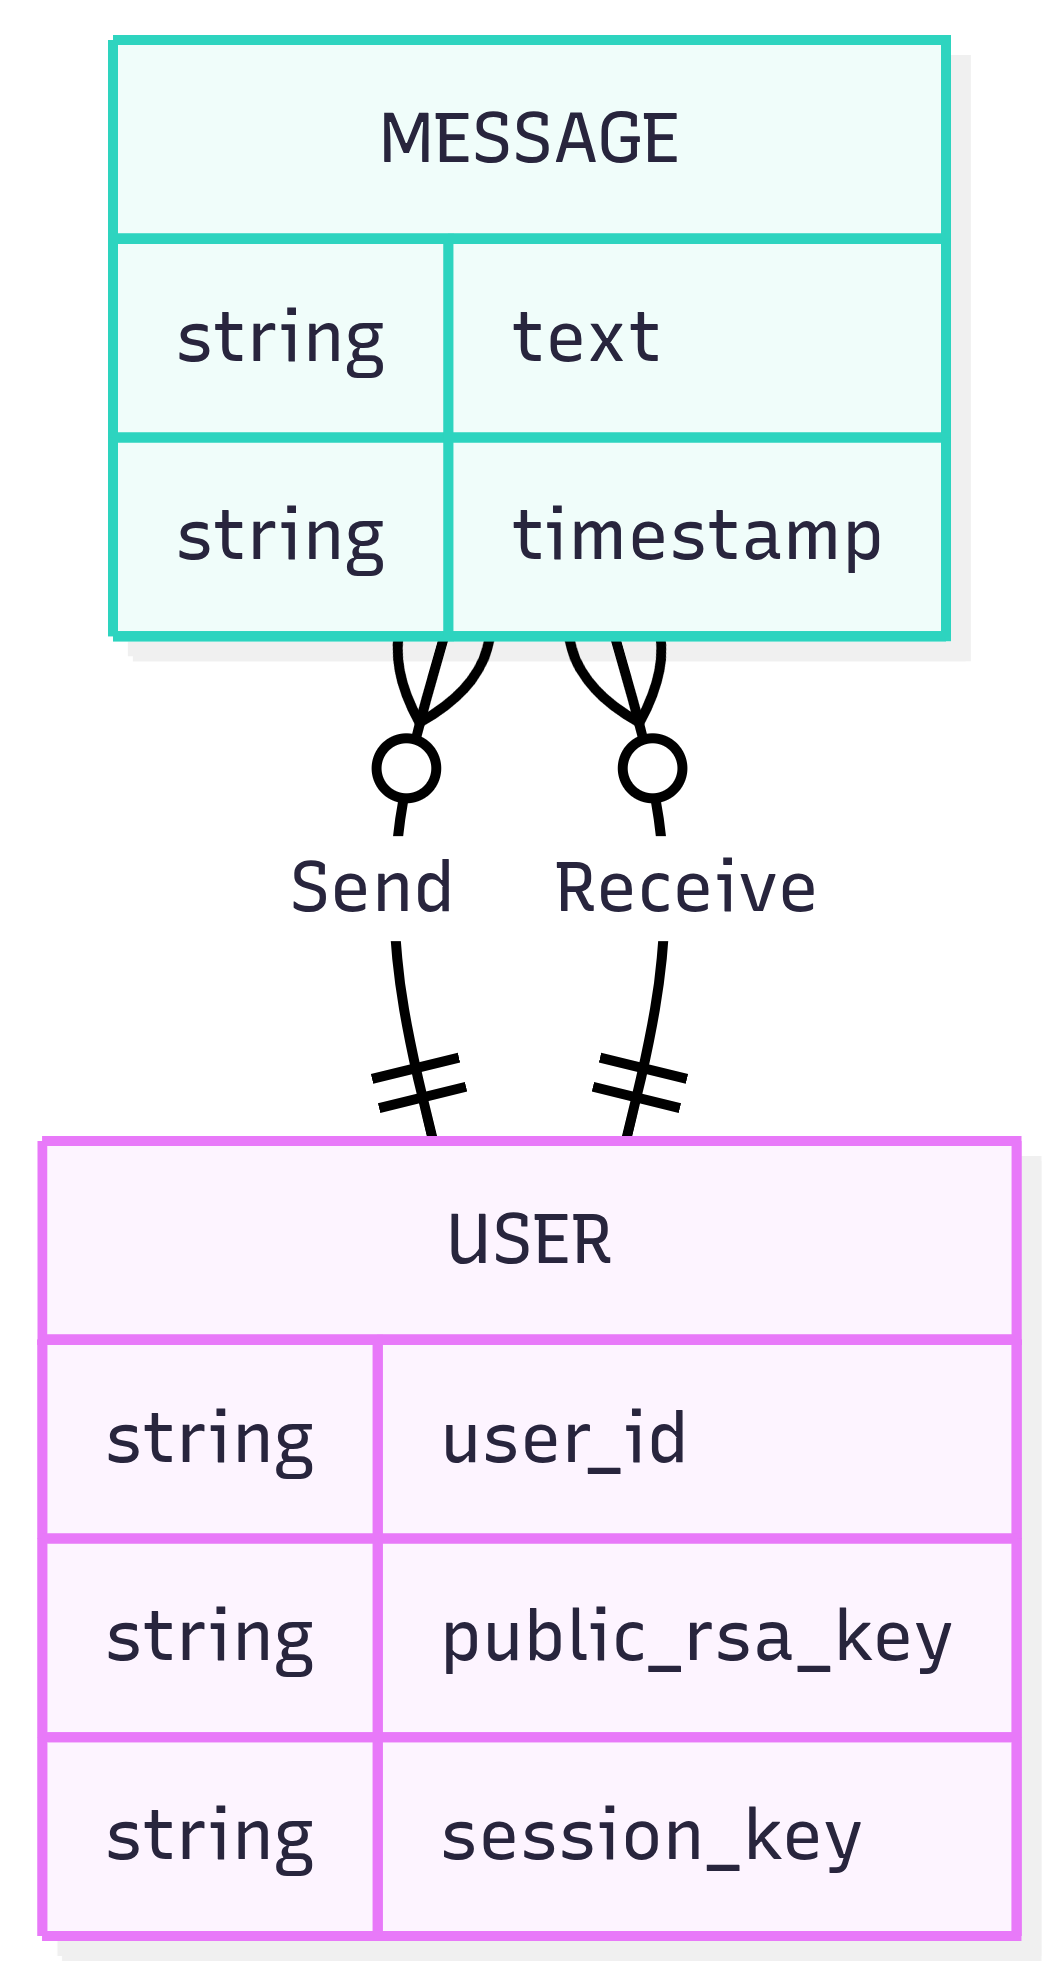
\includegraphics[width=.4\textwidth]{img/er/client_user_messages.png}
    \caption{Diagramma er database del client.}
    \label{er:client_db}
\end{figure}

Come si vede in \ref{er:client_db} il diagramma per i client e' molto simile a quello del server. Le
entita' sono le stesse ma cambiano i dati contenuti, in particolare per gli USERS non abbiamo l'hash
della password per ovvi motivi e nei MESSAGES manteniamo il messaggio in chiaro per evitare continue
decifrature al caricamento del db. Possiamo mantenere il testo in chiaro perche' se un
malintenzionato entra nel nostro PC avrebbe comunque accesso alle chiavi private e alle chiavi di
sessione con gli altri utenti quindi sarebbe tutto inutile.

Il client avra' inoltre una tabella local\_identity che contiene le cose personali quindi username e
chiavi pubbliche e private di RSA.

\section{Server}
In questa sezione vedremo il design del funzionamento del server.

\subsection{Message router}
Per cercare di rendere il codice pulito ho deciso di scrivere una classe router che permette di
registrare degli handler per specifiche tipologie di messaggi.

\begin{figure}[H]
    \centering{}
    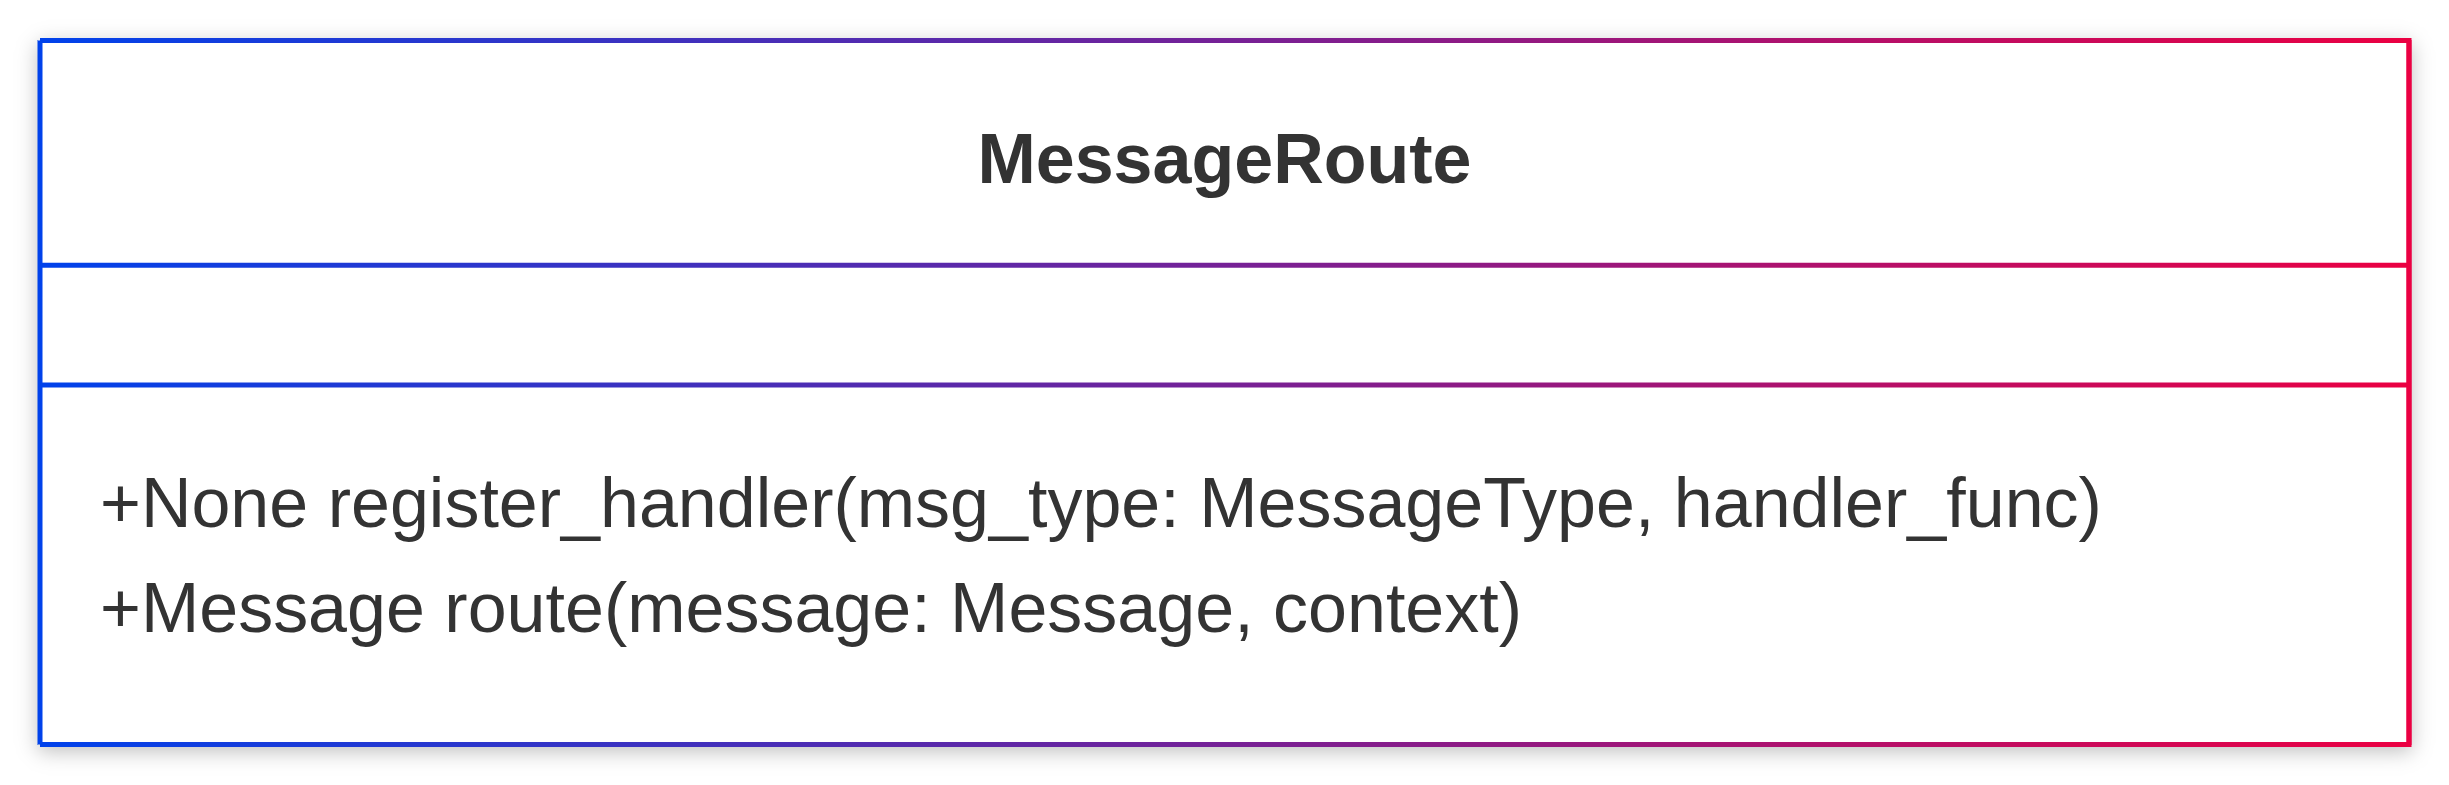
\includegraphics[width=.8\textwidth]{img/class/MessageRouter.png}
    \caption{Diagramma della classe MessageRouter.}
    \label{class:MessageRouter}
\end{figure}

Come si vede in \ref{class:MessageRouter} c'e' la possibilita' di registrare gli handlers e di
chiamare la funzione route che in base al context e al tipo di messaggio restituira' il messaggio di
risposta.

\subsubsection{Handlers}
Gli handlers sono semplici funzioni che preso un messaggio e un context eseguono l'azione richiesta
dai client. Ho definito i seguenti handlers:
\begin{itemize}
    \item register\_handler: gestisce l'azione di register di un nuovo user aggiungendolo al db
    verificando l'unicita' dell'username.
    \item login\_handler: gestisce il login degli utenti aggiornando il context.
    \item get\_messages\_handler: gestisce le richieste dei messaggi di tipo GET\_MESSAGES verificando
    che non ci siano accessi non autorizzati a messaggi.
    \item get\_public\_key\_handler: gestisce le richieste di tipo GET\_PUBLIC\_KEY.
    \item send\_message\_handler: gestisce le richieste di tipo SEND\_MESSAGE verificando che il sender
    sia effettivamente l'utente che ha fatto il login per evitare che qualcuno possa mandare
    messaggi per conto di altri.
\end{itemize}
Ogni handler restituisce un messaggio di risposta.

\subsection{Connection Handler}
Il ConnectionHandler e' colui che mantiene le connessioni con i vari client ed e' creato ad ogni
nuova connessione alla socket. Per ogni connessione c'e' un Thread che viene avviato sulla funzione
handle del ConnectionHandler, in questo modo posso facilmente gestire le sessioni perche' ogni
Thread ne rappresenta una e agisce in autonomia rispetto agli altri.

\begin{figure}[H]
    \centering{}
    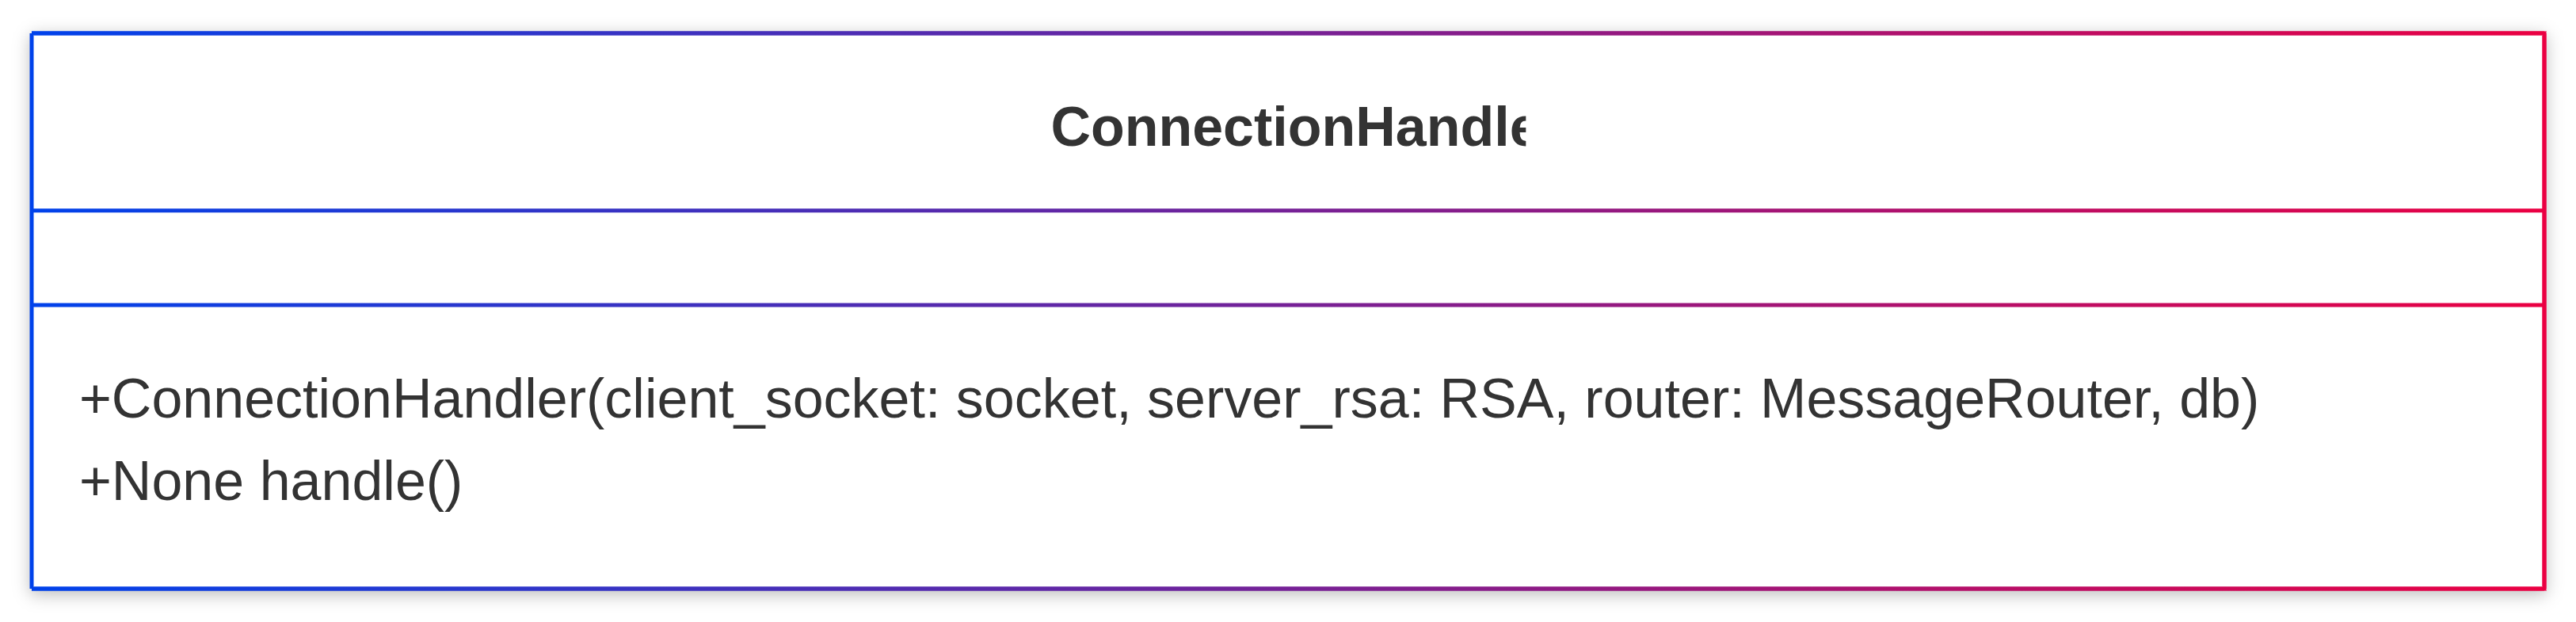
\includegraphics[width=.8\textwidth]{img/class/ConnectionHandler.png}
    \caption{Diagramma della classe ConnectionHandler.}
    \label{class:ConnectionHandler}
\end{figure}

Come si vede in \ref{class:ConnectionHandler} vi e' una funzione handle su cui partira' il Thread e
questa funzione eseguira' l'handshake e successivamente iniziera' il message loop in cui si
attendono i messaggi e si eseguono le rispettive azioni utilizzando il MessageRouter.

\section{Client}

\subsection{Server Connection}

\begin{figure}[H]
    \centering{}
    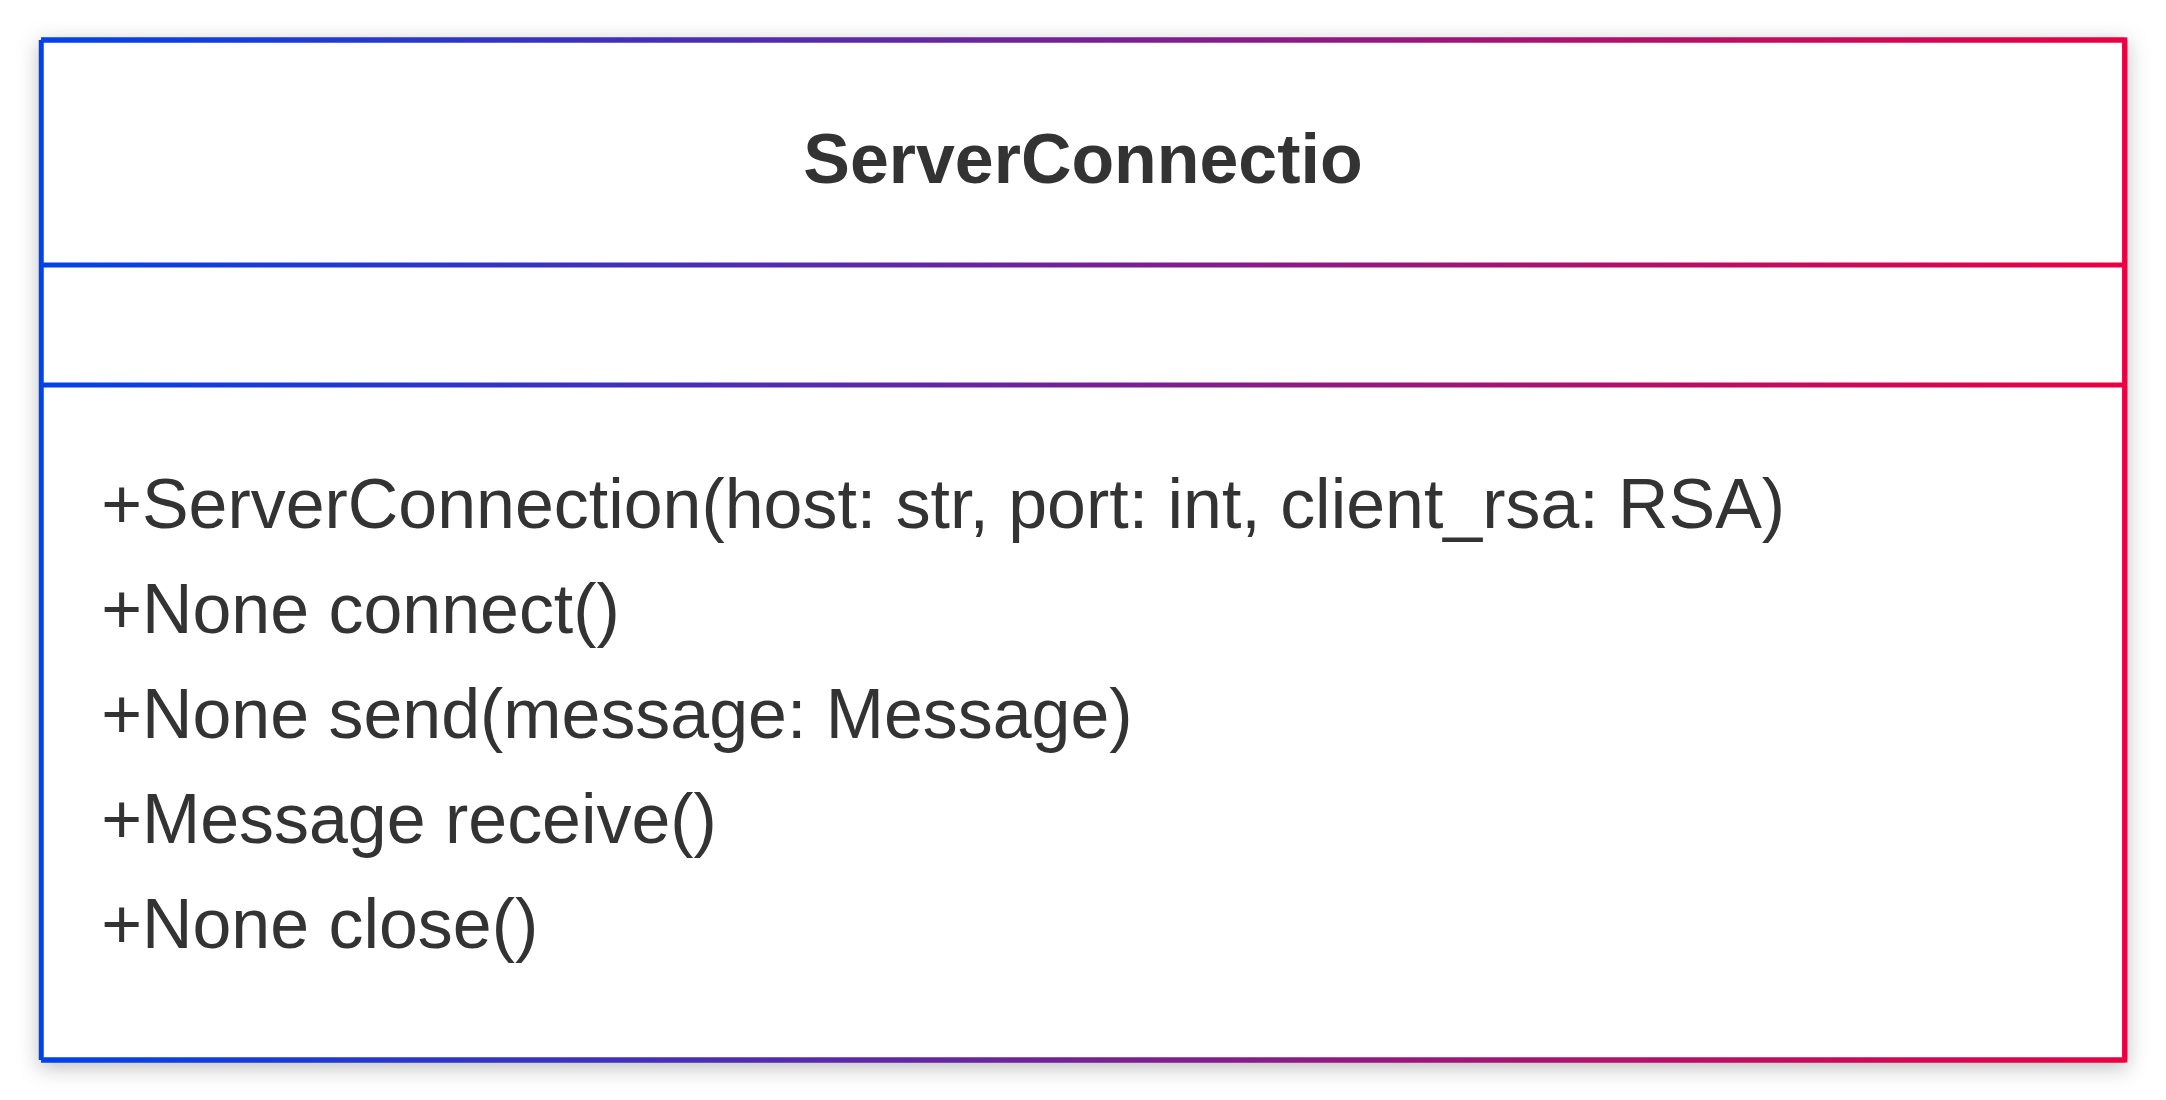
\includegraphics[width=.8\textwidth]{img/class/ServerConnection.png}
    \caption{Diagramma della classe ServerConnection.}
    \label{class:ConnectionHandler}
\end{figure}
La classe ServerConnection si occupa di mantenere la connessione TCP col server e si occupa
dell'invio e della ricezione dei messaggi in rete.

\subsection{Client}

\begin{figure}[H]
    \centering{}
    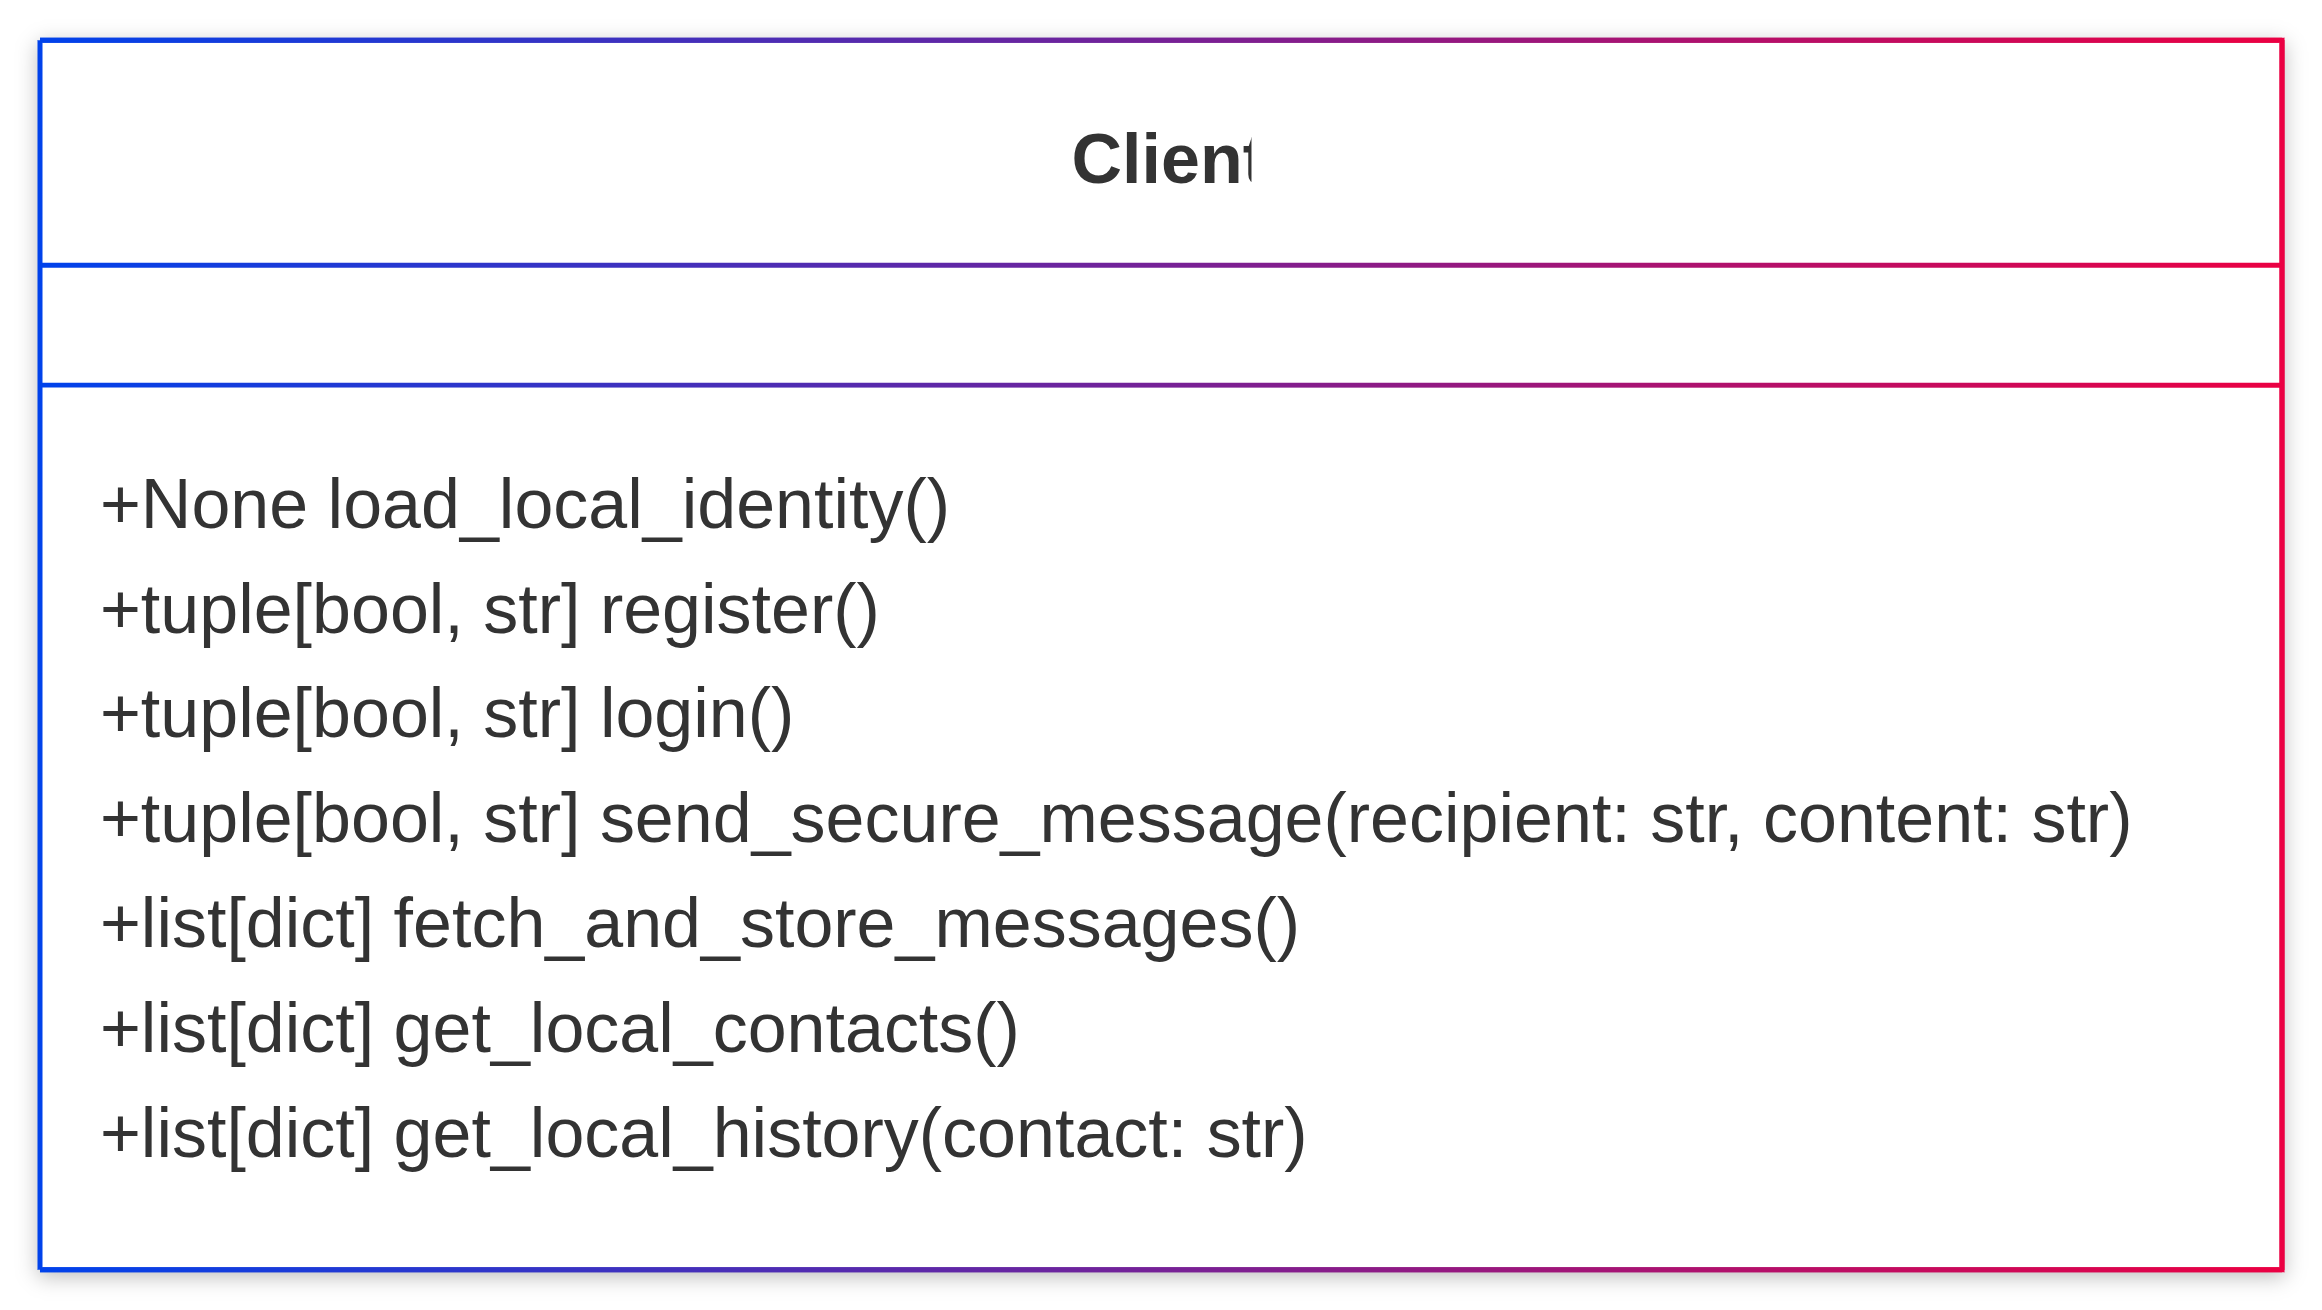
\includegraphics[width=.8\textwidth]{img/class/Client.png}
    \caption{Diagramma della classe Client.}
    \label{class:Client}
\end{figure}
La classe Client permette di eseguire tutte le istruzioni necessarie agli utenti come registrarsi,
eseguire il login, inviare messaggi ecc. Per l'invio dei messaggi al server utilizza una
ServerConnection.

\section{Configurazione e Costanti}
Come detto in precedenza la chiave pubblica del server e' nota a priori a tutti i client.
Anche per DH, p e g sono comuni a tutti ed ho deciso di utilizzare i valori forniti
\href{https://www.ietf.org/rfc/rfc3526.txt}{qui} per 2048 bit.

